%%%% kr-instructions.tex -- version 1.2 (27-Feb-2020)

\typeout{KR2020 Instructions for Authors}

% These are the instructions for authors for KR-20.

\documentclass{article}
\pdfpagewidth=8.5in
\pdfpageheight=11in

\usepackage{kr}

% Use the postscript times font!
\usepackage{times}
\usepackage{soul}
\usepackage{url}
\usepackage[hidelinks]{hyperref}
\usepackage[utf8]{inputenc}
\usepackage[small]{caption}
\usepackage{graphicx}
\usepackage{amsmath}
\usepackage{amsthm}
\usepackage{booktabs}
%\usepackage{algorithm}
%\usepackage{algorithmic}

\usepackage{enumerate}
\usepackage[linesnumbered,boxed]{algorithm2e}
\usepackage{amstext}
\usepackage{amssymb}
\usepackage{color}
%\usepackage{ulem}

\urlstyle{same}

% the following package is optional:
%\usepackage{latexsym}

% See https://www.overleaf.com/learn/latex/theorems_and_proofs
% for a nice explanation of how to define new theorems, but keep
% in mind that the amsthm package is already included in this
% template and that you must *not* alter the styling.
\newtheorem{example}{Example}
\newtheorem{theorem}{Theorem}

% Following comment is from ijcai97-submit.tex:
% The preparation of these files was supported by Schlumberger Palo Alto
% Research, AT\&T Bell Laboratories, and Morgan Kaufmann Publishers.
% Shirley Jowell, of Morgan Kaufmann Publishers, and Peter F.
% Patel-Schneider, of AT\&T Bell Laboratories collaborated on their
% preparation.

% These instructions can be modified and used in other conferences as long
% as credit to the authors and supporting agencies is retained, this notice
% is not changed, and further modification or reuse is not restricted.
% Neither Shirley Jowell nor Peter F. Patel-Schneider can be listed as
% contacts for providing assistance without their prior permission.

% To use for other conferences, change references to files and the
% conference appropriate and use other authors, contacts, publishers, and
% organizations.
% Also change the deadline and address for returning papers and the length and
% page charge instructions.
% Put where the files are available in the appropriate places.

\title{A Resolution Calculus for Forgetting in CTL}

% Single author syntax
\iffalse % (remove the multiple-author syntax below and \iffalse ... \fi here)
\author{%
    Author name
    \affiliations
    Affiliation
    \emails
    email@example.com    % email
}
\fi
% Multiple author syntax
\author{%
Renyan Feng$^{1,2}$\and
Erman Acar$^2$\and
Stefan Schlobach$^{2}$\and
Yisong Wang$^1$ \\
\affiliations
$^{1}$Guizhou University, P. R. China\\
$^{2}$Vrije Universiteit Amsterdam, Netherlands\\
%$^3$Third Affiliation\\
%$^4$Fourth Affiliation \\
\emails
fengrenyan@gmail.com,
\{k.s.schlobach, erman.acar\}@vu.nl,
yswang@gzu.edu.cn
}

\begin{document}

\newcommand{\tuple}[1]{{\langle{#1}\rangle}}
\newcommand{\Mod}{\textit{Mod}}
\newcommand\ie{{\it i.e. }}
\newcommand\eg{{\it e.g.}}
%\newcommand\st{{\it s.t. }}
\newtheorem{definition}{Definition}
%\newtheorem{examp}{Example}
%\newenvironment{example}{\begin{examp}\rm}{\end{examp}}
\newtheorem{lemma}{Lemma}
\newtheorem{proposition}{Proposition}
%\newtheorem{theorem}{Theorem}
\newtheorem{corollary}[theorem]{Corollary}
%\newenvironment{proof}{{\bf Proof:}}{\hfill\rule{2mm}{2mm}\\ }
\newcommand{\rto}{\rightarrow}
\newcommand{\lto}{\leftarrow}
\newcommand{\lrto}{\leftrightarrow}
\newcommand{\Rto}{\Rightarrow}
\newcommand{\Lto}{\Leftarrow}
\newcommand{\LRto}{\Leftrightarrow}
\newcommand{\Var}{\textit{Var}}
\newcommand{\Forget}{\textit{Forget}}
\newcommand{\KForget}{\textit{KForget}}
\newcommand{\TForget}{\textit{TForget}}
%\newcommand{\forget}{\textit{forget}}
\newcommand{\Fst}{\textit{Fst}}
\newcommand{\dep}{\textit{dep}}
\newcommand{\term}{\textit{term}}
\newcommand{\literal}{\textit{literal}}

\newcommand{\Atom}{\mathcal{A}}
\newcommand{\SFive}{\textbf{S5}}
\newcommand{\MPK}{\textsc{k}}
\newcommand{\MPB}{\textsc{b}}
\newcommand{\MPT}{\textsc{t}}
\newcommand{\MPA}{\forall}
\newcommand{\MPE}{\exists}

\newcommand{\DNF}{\textit{DNF}}
\newcommand{\CNF}{\textit{CNF}}

\newcommand{\degree}{\textit{degree}}
\newcommand{\sunfold}{\textit{sunfold}}

\newcommand{\Pos}{\textit{Pos}}
\newcommand{\Neg}{\textit{Neg}}
\newcommand\wrt{{\it w.r.t.}}
\newcommand{\Hm} {{\cal M}}
\newcommand{\Hw} {{\cal W}}
\newcommand{\Hr} {{\cal R}}
\newcommand{\Hb} {{\cal B}}
\newcommand{\Ha} {{\cal A}}

\newcommand{\Dsj}{\triangledown}

\newcommand{\wnext}{\widetilde{\bigcirc}}
\newcommand{\nex}{\bigcirc}
\newcommand{\ness}{\square}
\newcommand{\qness}{\boxminus}
\newcommand{\wqnext}{\widetilde{\circleddash}}
\newcommand{\qnext}{\circleddash}
\newcommand{\may}{\lozenge}
\newcommand{\qmay}{\blacklozenge}
\newcommand{\unt} {{\cal U}}
\newcommand{\since} {{\cal S}}
\newcommand{\SNF} {\textit{SNF$_C$}}
\newcommand{\start}{\textbf{start}}
\newcommand{\Elm}{\textit{Elm}}
\newcommand{\simp}{\textbf{simp}}
\newcommand{\nnf}{\textbf{nnf}}

\newcommand{\CTL}{\textrm{CTL}}
\newcommand{\Ind}{\textrm{Ind}}
\newcommand{\Tran}{\textrm{Tran}}
\newcommand{\Sub}{\textrm{Sub}}
\newcommand{\NI}{\textrm{NI}}
\newcommand{\Inst}{\textrm{Inst}}
\newcommand{\Com}{\textrm{Com}}
\newcommand{\Rp}{\textrm{Rp}}
\newcommand{\forget}{{\textsc{f}_\CTL}}
\newcommand{\ALL}{\textsc{a}}
\newcommand{\EXIST}{\textsc{e}}
\newcommand{\NEXT}{\textsc{x}}
\newcommand{\FUTURE}{\textsc{f}}
\newcommand{\UNTIL}{\textsc{u}}
\newcommand{\GLOBAL}{\textsc{g}}
\newcommand{\UNLESS}{\textsc{w}}
\newcommand{\Def}{\textrm{def}}
\newcommand{\IR}{\textrm{IR}}
\newcommand{\Tr}{\textrm{Tr}}
\newcommand{\dis}{\textrm{dis}}
\def\PP{\ensuremath{\textbf{PP}}}
\def\NgP{\ensuremath{\textbf{NP}}}
\def\W{\ensuremath{\textbf{W}}}
\newcommand{\Pre}{\textrm{Pre}}
\newcommand{\Post}{\textrm{Post}}


\newcommand{\CTLsnf}{{\textsc{SNF}_{\textsc{ctl}}^g}}
\newcommand{\ResC}{{\textsc{R}_{\textsc{ctl}}^{\succ, S}}}
\newcommand{\CTLforget}{{\textsc{F}_{\textsc{ctl}}}}
\newcommand{\Refine}{\textsc{Refine}}
\newcommand{\cf}{\textrm{cf.}}
\newcommand{\NEXP}{\textmd{\rm NEXP}}
\newcommand{\EXP}{\textmd{\rm EXP}}
\newcommand{\coNEXP}{\textmd{\rm co-NEXP}}
\newcommand{\NP}{\textmd{\rm NP}}
\newcommand{\coNP}{\textmd{\rm co-NP}}
\newcommand{\Pol}{\textmd{\rm P}}
\newcommand{\BH}[1]{\textmd{\rm BH}_{#1}}
\newcommand{\coBH}[1]{\textmd{\rm co-BH}_{#1}}
\newcommand{\Empty}{\varnothing}
\newcommand{\NLOG}{\textmd{\rm NLOG}}
\newcommand{\DeltaP}[1]{\Delta_{#1}^{p}}
\newcommand{\PIP}[1]{\Pi_{#1}^{p}}
\newcommand{\SigmaP}[1]{\Sigma_{#1}^{p}}

\maketitle

\begin{abstract}

Computation Tree Logic (CTL) is a popular logical formalism in computer science with a wide range of applications; it is used  in formal verification in the context of representing and reasoning about high-level system information (or \emph{specification}), but also in other domains e.g., planning.  Orthogonal to this, forgetting is the field of study which concerns removing information that is deemed irrelevant or obsolete from a knowledge base while guaranteeing certain properties.

In this paper, we present a resolution-based approach to perform \emph{forgetting} in \CTL.
%As we show, having such an approach let us perform forgetting while avoiding undesirable complications that arise from handling it on the semantic level.
More specifically, we develop a calculus which extends earlier work (\CTL\ with \emph{index} i.e., $\CTLsnf$) with additional rules i.e., EF-implication which connects \emph{next\ state} and \emph{future\ state}. As tailoring a resolution calculus for forgetting is a non-trivial task, our technical contribution is manifolded: ($i$) we provide a bisimulation between \CTL\ formulae and $\CTLsnf$ clauses; ($ii$) we introduce techniques for eliminating undesired atoms resulting from such transformation. Moreover, we show the soundness of our approach and analyse its computational complexity.


%Furthermore, it is shown that our algorithm is correct and the time and space complexity of our algorithm are $O((m+1)2^{4(n+n')}$.
%\keywords{Forgetting  \and CTL \and Model checking.}
\end{abstract}

%\begin{abstract}
%Computation Tree Logic (CTL) is one of the central formalisms in formal verification.
%This paper presents a resolution-based method for computing the forgetting in \CTL\, which has been proposed in another paper for KR this year.
%The method is an extension of the resolution calculus used to decide the satisfiability of \CTL\ formula.
%An important feature inherited from the satisfiability of resolution-based method is guided by transforming a \CTL\ formula into the normal form, i.e. %the set of $\CTLsnf$ clauses. The $\CTLsnf$ language extend \CTL\ with \emph{index} for Existential quantifier.
%We use binary bisimulation relation to relate \CTL\ and $\CTLsnf$, this shows that how to transform the \CTL\ formula into $\CTLsnf$ clauses and then %return to \CTL\ formula after finishing the computing process.
%Besides, we extend the original resolution rules by adding EF imply rules, which connects the \emph{next\ state} and \emph{future\ state}.
%Furthermore, it is shown that our algorithm is correct and the time and space complexity of our algorithm are $O((m+1)2^{4(n+n')}$.
%\keywords{Forgetting  \and CTL \and Model checking.}
%\end{abstract}

\section{Introduction}
%\emph{Model Checking} is an automatic, model-based, property-verification approach.
%In the past decades, it is not only  used in \emph{verification} but also in other domains e.g.,  \emph{planning}

Computation Tree Logic (\CTL)~\cite{clarke1981design} is one of the central logical formalisms in computer science with a wide range of applications; it is used mostly in formal verification in the context of representing and reasoning about high-level system information (or \emph{specification}), but also in other domains e.g., planning~\cite{giunchiglia1999planning,dal2002planning,akintunde2017planning}.
%In those cases, as the system or planning domain has been updated-some of the elements previously considered are no longer considered-if we have had those specifications, we do not need to reproduce the specifications that different from the original one only in that the latter using lesser atoms. Besides, with the size of the system or planning domain growing, not only the number of available (proposition) increased considerably, but also those specifications are often large in size and becoming more complex. This leads to the specification being difficult to maintain and modify, and costly to reuse for later processing, where only a specific part of an specification is of interest. All of this working directly on the whole of the original specification and building a new sub-specification are inadvisable. Therefore, a strong demand for techniques and automated tools for obtaining the specific sub-specification.
Both in planning and verification updates are required where, e.g., some of the elements previously considered are no longer required. In these cases it is desirable to update the specifications such that they contain only the relevant vocabulary without the need to fully reproduce them. Moreover, with increasing size of the systems or planning domains the formalization becomes prohibitively large in size and complexity. As a consequence specifications become overly difficult to maintain, modify and re-use for later processing overly costly, even if only a specific part of a specification is of interest. Therefore, techniques and automated tools for obtaining sub-specification based on restricted vocabularies are required.

\emph{Forgetting}, the task of distilling a reduced knowledge base that is relevant to a subset of the signature, addresses these issues.
As a logical notion, \emph{forgetting} was first formally defined
in propostional and first order-logics by Lin and Reiter~\cite{lin1994forget}.
Over the last twenty years, not only have researchers developed forgetting notions and theories in propositional and first-order logic, but also in other logic systems~\cite{eiter2019brief}, such as in logic programs under answer set/stable model semantics~\cite{DBLP:Zhang:AIJ2006,Eiter2008Semantic,Wong:PhD:Thesis,Yisong:KR:2012,Yisong:IJCAI:2013}, forgetting in description logic~\cite{Wang:AMAI:2010,Lutz:IJCAI:2011,zhao2017role} and in modal logic~\cite{Yan:AIJ:2009,Kaile:JAIR:2009,Yongmei:IJCAI:2011,fang2019forgetting}. Forgetting has been used in several application domains, such as planning~\cite{lin2003compiling},  conflict solving \cite{Lang2010Reasoning,Zhang2005Solving},
%knowledge compilation \cite{Zhang2009Knowledge,Bienvenu2010Knowledge},
creating restricted views of ontologies~\cite{zhao2017role},
%{ZhaoSchmidt18a},
strongest and weakest definitions \cite{Lang2008On}, SNC (WSC) \cite{DBLP:journals/ai/Lin01} and others.


%  Computation Tree Logic (\CTL)~\cite{clarke1981design} is one of the main logical formalisms for
% program specification and verification.
%Computation Tree Logic (\CTL)~\cite{clarke1981design} is one of the central logical formalisms in computer science with a wide-range of applications; it is used mostly in formal verification in the context of representing and reasoning about high-level system information (or \emph{specification}), but also in other domains e.g., planning.
Although forgetting has been extensively investigated from various aspects of different logical systems,
%these existing forgetting methods in propositional
%logic, answer set programming, description logic and modal logic
it is not directly applicable to \CTL\ knowledge bases.
%Similar with that in~\cite{Yan:AIJ:2009}, we have studied the forgetting in \CTL\ from the semantic forgetting point of view in ``the theory paper".
%And it is shown that our definition of forgetting satisfies those four postulates of forgetting.
% Although we have proposed an model-based approach to compute forgetting in \CTL\ in ``the theory paper", but both time and space complexity are 2-exponential. It is urgent to find an efficient algorithm.
There are a number of challenges. For instance, in propositional forgetting theory, forgetting atom $q$ from $\varphi$ is equivalent to a formula $\varphi[q/\top] \vee \varphi[q/\perp]$, where $\varphi[q/X]$ is a formula obtained from $\varphi$ by replacing each $q$ with $X$ ($X\in \{\top, \perp\}$).
This method cannot be extended to \CTL. Consider a \CTL\ formula $\psi=\ALL\GLOBAL p \wedge \neg \ALL\GLOBAL q \wedge \neg \ALL\GLOBAL \neg q$. If we want to forget
atom $q$ from $\psi$ by using the above method, we would have $\psi[q/\top] \vee \psi[q/\perp] \equiv \perp$. This is obviously not correct since after forgetting $q$ this specification should not become inconsistent.
%Besides, we also cannot use the method in modal logic since there is
%Another example is computing the result of forgetting $p$ from $\ALL((p\wedge q) \UNTIL (f\vee m)) \wedge r$.

%For another, as far as I know the existing methods to compute forgetting include the classical one talked above and resolution-based approaches in propositional

Another problem is that resolution based methods for propositional logic~\cite{lin1994forget,Yisong:2015:arx} and Ackermann-based approach (second-order elimination) in description logic~\cite{Zhao:2017:IJCAI} require a specific normal form which does not exist in this form in \CTL.
While any \CTL\ formula can be transformed into a set of $\CTLsnf$ clauses, which is a variant of \CTL\ for which such a normal form does exist, it introduces \emph{indices} and extra atoms. Both these two problems will have to be addressed.

In this paper, we give the definition of forgetting in \CTL\ from the semantic forgetting point of view and explore a resolution-based method to compute it. In particular, we extend the Resolution Calculus in~\cite{zhang2014resolution} by eliminating the atoms introduced in the transformation process %and combining the \CTL\ with $\CTLsnf$
by using a \emph{binary bisimulation relation} (one on the set of atoms, one on indices).
Such a bisimulation relation is an extension of the set-based bisimulation introduced in \cite{renyansfirstpaper} by taking \emph{index} into account.

In Section 2 we introduce the notation and technical preliminaries.
In Section 3 we give a more precise definition of the forgetting problem.
As key contributions, Section 4, introduces the resolution-based approach, as well as the proofs of soundness and complexity.
We conclude the paper with some related and future work, as well as a brief discussion. Due to space restrictions and to avoid hindering the flow of content, some of the proves are moved to the supplementary material~\footnote{https://github.com/fengrenyan/Resolution-proof-CTL.git}.
%
%
\section{Preliminaries}
We start with some technical and notational preliminaries. Throughout this paper we fix a finite set $\Ha$ of propositional variables (or atoms), and use $V$, $V'$ for subsets of $\Ha$.
% In the following several parts, we will introduce the structure we will use for \CTL, syntax and semantic of \CTL\ and the normal form $\CTLsnf$ (Separated Normal Form with Global Clauses for \CTL) of \CTL~\cite{zhang2009refined}.
\subsection{Model structure in \CTL}
 In general, a transition system
%\footnote{According to \cite{Baier:PMC:2008},
%a {\em transition system} TS is a tuple $(S, Act,\rto,I, AP, L)$ where
%(1) $S$ is a set of states,
%(2) $\textrm{Act}$ is a set of actions,
%(3) $\rto\subseteq S\times \textrm{Act}\times S$ is a transition relation,
%(4) $I\subseteq S$ is a set of initial states,
%(5) $\textrm{AP}$ is a set of atomic propositions, and
%(6) $L:S\rto 2^{\textrm{AP}}$ is a labeling function.}
 can be described by a \emph{model\ structure} (or \emph{Kripke \ structure}) (see~\cite{Baier:PMC:2008} for details). A model structure is a triple $\Hm=(S,R,L)$, where
\begin{itemize}
  \item $S$ is a finite nonempty set of states, % \footnote{Indeed, every state is identified by a configuration of atoms i.e., which holds in that state.},
  \item $R\subseteq S\times S$ and, for each $s\in S$, there
  is $s'\in S$ such that $(s,s')\in R$,
  \item $L: S\rto 2^{\cal A}$ is a labeling function.
\end{itemize}
%We call a model structure $\Hm$ on a set $V$ of atoms if $L: S \rto 2^V$, i.e., the labelling function $L$ map every state to $V$ (not the $\Ha$).
Given a model structure $\Hm=(S,R,L)$, a \emph{path} $\pi_{s_i}$ starting from $s_i$ of $\Hm$ is an infinite sequence of states $\pi_{s_i}=(s_i, s_{i+1} s_{i+2},\dots)$, where for each $j$ ($0\leq i\leq j$), $(s_j, s_{j+1}) \in R$. By $s'\in \pi_{s_i}$ we mean that $s'$ is a state in the path $\pi_{s_i}$.
A state $s\in S$ is {\em initial} if for any state $s'\in S$, there is a path $\pi_s$ s.t $s'\in \pi_s$.
If $s_0$ is an initial state of $\Hm$, then we denote this model structure $\Hm$ as $(S,R,L,s_0)$.

For a given model structure $\Hm=(S,R,L,s_0)$ and $s\in S$,
the {\em computation tree}
$\Tr_n^{\cal M}(s)$ of $\cal M$ (or simply $\Tr_n(s)$), that has depth $n \ge 0$ and is rooted at $s$, is recursively defined \cite{DBLP:journals/tcs/BrowneCG88} as follows:
\begin{itemize}
  \item $\Tr_0(s)$ consists of a single node $s$ with label $s$.
  \item $\Tr_{n+1}(s)$ has as its root a node $m$ with label  $s$, and
  if $(s,s')\in R$ then the node $m$ has a subtree $\Tr_n(s')$.
 % \footnote{Though
%  some nodes of the tree may have the same label, they are different nodes in the tree.}.
\end{itemize}
%By $s_n$ we mean a $n$th level node of tree $\Tr_m(s)$ $(m \geq n)$.

A {\em \MPK-structure} (or {\em \MPK-interpretation}) is a model structure
${\cal M}=(S, R, L, s_0)$ associating
with a state $s\in S$, which is written as $({\cal M},s)$ for convenience in the following.
In case $s=s_0$ is an initial state of $\cal M$, the \MPK-structure is {\em initial}.



\subsection{Syntax and Semantics of \CTL}
In the following, we briefly review the basic syntax and semantics
of the \CTL~\cite{DBLP:journals/toplas/ClarkeES86}.
The {\em signature} of the language $\cal L$ of \CTL\ includes:
\begin{itemize}
  \item a finite set of Boolean variables, called {\em atoms} of $\cal L$: $\cal A$;
  \item constant symbols: $\bot$ and $\top$;
  \item the classical connectives: $\lor$ and $\neg$;
  %\item the propositional constants: $\bot$;
  \item the path quantifiers: $\ALL$ and $\EXIST$;
  \item the temporal operators: \NEXT, \FUTURE, \GLOBAL, \UNTIL\ and \UNLESS, that
  means `neXt state', `some Future state', `all future states (Globally)', `Until' and `Unless', respectively;
  \item parentheses: ( and ).
\end{itemize}

The {\em (existential normal form or ENF in short) formulas} of
$\cal L$ are inductively defined via a Backus Naur form:
\begin{equation}\label{def:CTL:formulas}
  \phi ::=  \bot \mid \top \mid p \mid\neg\phi \mid \phi\lor\phi \mid
    \EXIST \NEXT \phi \mid
    %\EXIST \FUTURE \phi \mid
    \EXIST \GLOBAL \phi \mid
    \EXIST [\phi\ \UNTIL\ \phi]%.% \mid
    %\ALL \NEXT \phi \mid
%    \ALL \FUTURE \phi \mid
%    \ALL \GLOBAL \phi \mid
%    \ALL [\phi\ \UNTIL\ \phi]
\end{equation}
where $p\in\cal A$. The formulas $\phi\land\psi$ and $\phi\supset \psi$
are defined in the usual way.
Other formulas in $\cal L$ are abbreviated
using the forms in (\ref{def:CTL:formulas}).
%Notice that, according to the
%above definition for formulas of \CTL,
%each of the \CTL\ {\em temporal connectives} has the form $XY$
%where $X\in \{\ALL,\EXIST\}$ and  $Y\in\{\NEXT, \FUTURE, \GLOBAL, \UNTIL\}$.
%The priorities for the \CTL\ connectives are assumed to be (from the highest to the lowest):
%\begin{equation*}
 % \neg, \EXIST\NEXT, \EXIST\FUTURE, \EXIST\GLOBAL, \ALL\NEXT, \ALL\FUTURE, \ALL\GLOBAL
 % \prec \land \prec \lor \prec \EXIST\UNTIL, \ALL\UNTIL, \EXIST \UNLESS, \ALL \UNLESS, \rto.
%\end{equation*}

Next, we define the semantics.
Let ${\cal M}=(S,R,L,s_0)$ be a model structure, $s\in S$ and $\phi \in \cal L$.
The {\em satisfiability} relationship between $({\cal M},s)$ and $\phi$,
written $({\cal M},s)\models\phi$, is inductively defined on the structure of $\phi$ as follows:

\begin{itemize}
  \item $({\cal M},s)\not\models\bot$ \text{ and }  $({\cal M},s)\models\top$;
  \item $({\cal M},s)\models p$ iff $p\in L(s)$;
  \item $({\cal M},s)\models \phi_1\lor\phi_2$ iff
    $({\cal M},s)\models \phi_1$ or $({\cal M},s)\models \phi_2$;
  \item $({\cal M},s)\models \neg\phi$ iff  $({\cal M},s)\not\models\phi$;
  \item $({\cal M},s)\models \EXIST\NEXT\phi$ iff
    $({\cal M},s_1)\models\phi$ for some $s_1\in S$ and $(s,s_1)\in R$;
  \item $({\cal M},s)\models \EXIST\GLOBAL\phi$ iff
    $\cal M$ has a path $(s_1=s,s_2,\ldots)$ such that
    $({\cal M},s_i)\models\phi$ for each $i\ge 1$;
  \item $({\cal M},s)\models \EXIST[\phi_1\UNTIL\phi_2]$ iff
    $\cal M$ has a path $(s_1=s,s_2,\ldots)$ such that, for some $i\ge 1$,
    $({\cal M},s_i)\models\phi_2$ and
    $({\cal M},s_j)\models\phi_1$ for each $1\leq j<i$.
\end{itemize}

Similar to the work in \cite{DBLP:journals/tcs/BrowneCG88,Bolotov:1999:JETAI},
only initial \MPK-structures are considered to be candidate models
in the following, unless otherwise noted. Formally,
an initial \MPK-structure $\cal K$ is a {\em model} of a formula (or set of formulas) $\phi$
whenever ${\cal K}\models\phi$ (or ${\cal K} \models \psi$ for each $\psi\in \varphi$).
%Let $\Pi$ be a set of formulae, ${\cal K} \models \Pi$ if for each $\phi\in \Pi$ there is $\cal K \models \phi$.
We denote $\Mod(\phi)$ the set of models of $\phi$.
%The formula
$\phi$  is {\em satisfiable}
if $\Mod(\phi)\neq\emptyset$.
Given two formulas (or sets of formulas) $\phi_1$ and $\phi_2$,  $\phi_1\models\phi_2$ we mean $\Mod(\phi_1)\subseteq\Mod(\phi_2)$. And
by $\phi_1\equiv\phi_2$, we mean $\phi_1\models\phi_2$ and $\phi_2\models\phi_1$.
In this case, $\phi_1$ is {\em equivalent} to $\phi_2$.
The set of atoms occurring in $\phi_1$ is denoted by $\Var(\phi_1)$.
The formula $\phi_1$ is {\em irrelevant to} the atoms in a set $V$ (or simply $V$-{\em irrelevant}), written $\IR(\phi_1,V)$,
if there is a formula $\psi$ with
$\Var(\psi)\cap V=\emptyset$ such that $\phi_1\equiv\psi$.
The $V$-{\em irrelevant} of a set of formulas can be defined similarly.
% Similar to the work in \cite{DBLP:journals/tcs/BrowneCG88,Bolotov:1999:JETAI},
% only initial \MPK-structures are considered to be candidate models
% in the following, unless otherwise noted. Formally,
% an initial \MPK-structure $\cal K$ is a {\em model} of a formula $\phi$
% whenever ${\cal K}\models\phi$.
% %Let $\Pi$ be a set of formulae, ${\cal K} \models \Pi$ if for each $\phi\in \Pi$ there is $\cal K \models \phi$.
% We denote $\Mod(\phi)$ the set of models of $\phi$.
% The formula $\phi$  is {\em satisfiable}
% iff $\Mod(\phi)\neq\emptyset$.
% Given two formulas $\phi_1$ and $\phi_2$, by $\phi_1\models\phi_2$, we mean $\Mod(\phi_1)\subseteq\Mod(\phi_2)$, and
% by $\phi_1\equiv\phi_2$, we mean $\phi_1\models\phi_2$ and $\phi_2\models\phi_1$.
% In this case, $\phi_1$ is {\em equivalent} to $\phi_2$.
% The set of atoms occurring in $\phi_1$, is denoted by $\Var(\phi_1)$. We say that
%  $\phi_1$ is $V$-{\em irrelevant}, and write $\IR(\phi_1,V)$,
% if there is a formula $\psi$ with
% $\Var(\psi)\cap V=\emptyset$ such that $\phi_1\equiv\psi$.


\subsection{The Normal Form of \CTL}
It is  known that any \CTL\ formula $\varphi$ can be transformed into a set $T_\varphi$ of $\CTLsnf$ (Separated Normal Form with Global Clauses for \CTL) clauses in polynomial time such that $\varphi$ is satisfiable iff $T_\varphi$ is satisfiable~\cite{zhang2008first}.
An important difference between \CTL\ formulae and $\CTLsnf$ is that $\CTLsnf$ is an extension of the syntax of \CTL\ to use indices. These indices can be used to preserve a particular path context. The language of $\CTLsnf$ clauses is defined over an extension of \CTL. That is, the language is based on: (1) the language of CTL; (2) a propositional constant $\start$; (3) a countably infinite index set $\Ind$; and (4) temporal operators: $\EXIST_{\tuple{ind}} \NEXT$, $\EXIST_{\tuple{ind}} \FUTURE$, $\EXIST_{\tuple{ind}} \GLOBAL$, and $\EXIST_{\tuple{ind}} \UNTIL$. 

% and $\EXIST_{\tuple{ind}} \UNLESS$.

%The priorities for the $\CTLsnf$\ connectives are assumed to be (from the highest to the lowest):
%\begin{align*}
%  &\neg, (\EXIST\NEXT,\EXIST_{\tuple{ind}}\NEXT), (\EXIST\FUTURE ,\EXIST_{\tuple{ind}}\FUTURE), (\EXIST\GLOBAL,\EXIST_{\tuple{ind}} \GLOBAL), \ALL\NEXT, \ALL\FUTURE, \ALL\GLOBAL \\
%  &\prec \land \prec \lor \prec (\EXIST\UNTIL,\EXIST_{\tuple{ind}} \UNTIL), \ALL\UNTIL, (\EXIST \UNLESS, ,\EXIST_{\tuple{ind}}\UNLESS), \ALL \UNLESS, \rto.
%\end{align*}
%Where the operators in the same brackets have the same priority.

%The $\CTLsnf$ clauses consists of formulae of the following forms: $\ALL \GLOBAL(\start \supset \bigvee_{j=1}^k m_j)$ (initial clause), $\ALL \GLOBAL(true \supset \bigvee_{j=1}^k m_j)$ (global clause), $\ALL \GLOBAL(\bigwedge_{i=1}^n l_i \supset \ALL \NEXT \bigvee_{j=1}^k m_j)$ (\ALL-step clause), $\ALL \GLOBAL(\bigwedge_{i=1}^n l_i \supset \EXIST_\tuple{ind} \NEXT \bigvee_{j=1}^k m_j)$ (\EXIST-step clause), $\ALL \GLOBAL(\bigwedge_{i=1}^n l_i \supset \ALL \FUTURE l)$ (\ALL-sometime clause) and $\ALL \GLOBAL(\bigwedge_{i=1}^n l_i \supset \EXIST_{\tuple{ind}} \FUTURE l)$ (\EXIST-sometime clause),
We introduce the $\CTLsnf$ clauses first, then we talk about its semantics. A $\CTLsnf$ clause consists of formulae of the following forms.
\begin{align*}
& \ALL \GLOBAL(\start \supset \bigvee_{j=1}^k m_j) && (initial\ clause) \\
& \ALL \GLOBAL(true \supset \bigvee_{j=1}^k m_j) && (global\ clause) \\
& \ALL \GLOBAL(\bigwedge_{i=1}^n l_i \supset \ALL \NEXT \bigvee_{j=1}^k m_j) && (\ALL-step\ clause)\\
& \ALL \GLOBAL(\bigwedge_{i=1}^n l_i \supset \EXIST_\tuple{ind} \NEXT \bigvee_{j=1}^k m_j) && (\EXIST-step\ clause)\\
& \ALL \GLOBAL(\bigwedge_{i=1}^n l_i \supset \ALL \FUTURE l) && (\ALL-sometime\ clause)\\
& \ALL \GLOBAL(\bigwedge_{i=1}^n l_i \supset \EXIST_{\tuple{ind}} \FUTURE l) && (\EXIST-sometime\ clause).
\end{align*}
where $k \ge 0$, $n > 0$, $\start$ is a propositional constant, $l_i$ ($1 \le i \le n$), $m_j$ ($1 \le j \le k$) and $l$ are literals, that is, atomic propositions or their negation, and $ind\in \Ind$. %(Ind is a countably infinite index set).
By a clause, we mean the classical clause or the $\CTLsnf$ clause unless explicitly stated.
As all clauses are of the form $\ALL \GLOBAL(P \supset D)$ , we often simply write $P \supset D$ instead.
 %A set $T$ of $\CTLsnf$ clauses is satisfiable if there is a model $\Hm=(S, R, L, [\_], s_0)$ \st\ for all clause $C\in T$, $(\Hm, s_0) \models C$.

Formulae of $\CTLsnf$ over $\Ha$ are interpreted in \Ind-model structure $\Hm=(S,R,L, [\_], s_0)$, where $S$, $R$, $L$ and $s_0$ is the same as our model structure talked above and $[\_]: \Ind \rto 2^{(S*S)}$ maps every index $ind \in \Ind$ to a successor function $[ind]$ which is a functional relation on $S$ and a subset of the binary accessibility relation $R$. That is, for every $s\in S$ there exists exactly a state $s'\in S$ such that $(s,s')\in [ind]$ and $(s,s')\in R$.
%In this paper we do not need a strict tree model structure as in~\cite{zhang2009refined}, that is we do not those restrictions on $s_0$ due to that only for simplifying the proof but do not impact the satisfiability of a formula~\cite{zhang2009refined}.
An infinite path $\pi_{s_i}^{\tuple{ind}}$ is an infinite sequence of states $s_i, s_{i+1}, s_{i+2},\dots$ such that for every $j\geq i$, $(s_j, s_{j+1})\in [ind]$.
%Let $\pi$ be a path in \Ind-model structure $\Hm$, by $s\in \pi$ we mean that $s$ is a state in the path $\pi$.

Similarly, an {\em \Ind-structure} (or {\em \Ind-interpretation}) is an \Ind-model structure
${\cal M}=(S, R, L, [\_], s_0)$ associating
with a state $s\in S$, which is simplified as $({\cal M},s)$ for convenience in the following.
In the case that $s$ is an initial state of $\cal M$, the \Ind-structure is {\em initial}.

%The semantics of $\CTLsnf$ is an extension of the semantics of \CTL\ defined in Section 2.2 except using the \Ind-model structure $\Hm=(S,R,L,[\_],s_0)$ replace model structure, $({\cal M},s_i) \models \start$ iff $s_i=s_0$ and for all $\EXIST_{\tuple{ind}} \Gamma$ are explained in the path $\pi_{s_i}^{\tuple{ind}}$, where $\Gamma\in \{\NEXT, \GLOBAL, \UNTIL,\UNLESS\}$.
The semantics of $\CTLsnf$ is then
defined as an extension of the semantics of \CTL.
% Let $\varphi$ and $\psi$ be two $\CTLsnf$ formulae, $\Hm=(S,R,L,[\_],s_0)$ be an \Ind-model structure and $s_i \in S$. The relation ``$\models$" between $\CTLsnf$ formulae and $(\Hm,s_i)$ is defined recursively as follows:
Let ${\cal M}=(S,R,L,[\_],s_0)$ be an \Ind-model structure, $s_i\in S$ and $\psi$ a $\CTLsnf$ formulae.
The {\em satisfiability} relationship between $({\cal M},s_i)$ and $\psi$,
written $({\cal M},s_i)\models\psi$, is inductively defined on the structure of $\psi$ as follows:
\begin{itemize}
  \item $({\cal M},s_i) \models \start$ iff $s_i=s_0$;
  \item $({\cal M},s_i)\models \EXIST_{\tuple{ind}} \NEXT \psi$ iff for the path $\pi_{s_i}^{\tuple{ind}}$, $(\Hm, s_{i+1})\models \psi$;
  \item $({\cal M},s_i)\models \EXIST_{\tuple{ind}}\GLOBAL\psi$ iff
    for every $s_j \in \pi_{s_i}^{\tuple{ind}}$,
    $(\Hm,s_j) \models \psi$;
  \item $({\cal M},s_i)\models \EXIST_{\tuple{ind}}[\psi_1\UNTIL\psi_2]$ iff
      there exists $s_j\in \pi_{s_i}^{\tuple{ind}}$ such that $(\Hm,s_j) \models \psi_2$ and for every $s_k \in \pi_{s_i}^{\tuple{ind}}$, if $i\leq k < j$, then $(\Hm,s_k) \models \psi_1$;
  \item $(\Hm,s_i) \models \EXIST_{\tuple{ind}} \FUTURE \psi$ iff $(\Hm,s_i) \models \EXIST_{\tuple{ind}}[\top \UNTIL\psi]$.
  %\item $({\cal M},s_i)\models \EXIST_{\tuple{ind}}[\varphi\UNLESS\psi]$ iff $(\Hm,s_i) \models \EXIST_{\tuple{ind}}\GLOBAL \varphi$ or $({\cal M},s_i)\models \EXIST_{\tuple{ind}}[\varphi\UNTIL\psi]$.
\end{itemize}
The semantics of the remaining operators are analogous to that of \CTL\ given previously.
%but in the extended \Ind-model structure ${\cal M}=(S, R, L, [\_],s_0)$.
A $\CTLsnf$ formula $\varphi$ is satisfiable, iff for some \Ind-model structure $\Hm=(S,R,L,[\_],s_0)$, $(\Hm,s_0)\models \varphi$, and unsatisfiable otherwise. And if $(\Hm,s_0)\models \varphi$ then $(\Hm,s_0)$ is called an \Ind-model of $\varphi$, and we say that $(\Hm,s_0)$ satisfies $\varphi$.
By $T \wedge \varphi$ we mean $\bigwedge_{\psi\in T} \psi \wedge \varphi$, where $T$ is a finite set of formulae.
Other terminologies are similar with those in Section 2.2.




\section{Problem Definition}
% In this section we will introduce forgetting based on the notion of $V$-bisimulation.
% Intuitively, bisimulation relates states that mutually mimic all individual transitions~\cite{Baier:PMC:2008}. While the $V$-bisimulation relates states that mutually mimic all individual transitions on $\Ha - V$, this is close with forgetting some set $V$ of atoms.
The concept of semantic forgetting in \CTL\ was introduced formally in~\cite{renyansfirstpaper}. We recall the main results that are required for this paper.
To present a formal definition of knowledge forgetting, we need the concepts of V-bisimulation on a given signature. It is (somehow) an extension of the classical bisimulation for \CTL\ in \cite{Baier:PMC:2008}.

For convenience, in the following we denote $\Hm=(S, R, L, s_0)$,
$\Hm'=(S',R',L',s_0')$, $\Hm_i=(S_i, R_i,L_i, s_0^i)$ (or $\Hm=(S, R, L, [\_], s_0)$,
$\Hm'=(S',R',L', [\_],s_0')$, $\Hm_i=(S_i, R_i,L_i, [\_], s_0^i)$) and ${\cal K}_i=(\Hm_i, s_i)$ with $s_i \in S_i$
and $i \in \mathbb{N}$.

Let
${\cal K}_i=({\cal M}_i,s_i)$ with $i\in\{1,2\}$,
\begin{itemize}
  \item $({\cal K}_1,{\cal K}_2)\in\Hb_0$ if $L_1(s_1)- V=L_2(s_2)- V$;  % and ${\cal K}'=(\tuple{S', R',L'},s')$;
  \item for $n\ge 0$, $({\cal K}_1,{\cal K}_2)\in\Hb_{n+1}$ if:
  \begin{itemize}
    \item $({\cal K}_1,{\cal K}_2)\in\Hb_0$,
    \item for every $(s_1,s_1')\in R_1$, there is a $(s_2,s_2')\in R_2$
    such that $({\cal K}_1',{\cal K}_2')\in \Hb_n$, and
    \item for every $(s_2,s_2')\in R_2$, there is a $(s_1,s_1')\in R_1$
    such that $({\cal K}_1',{\cal K}_2')\in \Hb_n$,
  \end{itemize}
  where ${\cal K}_i'=({\cal M}_i,s_i')$ with $i\in\{1,2\}$.
\end{itemize}

Now, we define the notion of $V$-bisimulation between \MPK-structures:
\begin{definition}[$V$-bisimulation] %~\cite{renyansfirstpaper}
  \label{def:V-bisimulation}
   Let $V\subseteq\cal A$. Two \MPK-structures (or \Ind-structures) ${\cal K}_1$ and ${\cal K}_2$ are $V$-{\em bisimilar},  denoted ${\cal K}_1 \lrto_V {\cal K}_2$,
 if and only if $({\cal K}_1,{\cal K}_2)\in {\Hb_i}\mbox{ for all }i\ge 0.$ Moreover, two paths $\pi_i=(s_{i,1},s_{i,2},\ldots)$ of $\Hm_i$ with $i\in \{1,2\}$
 are $V$-{\em bisimilar} if
$ {\cal K}_{1,j} \lrto_V {\cal K}_{2,j}\mbox { for every $j\ge 1$ }$
 where ${\cal K}_{i,j}=(\Hm_i,s_{i,j})$.
\end{definition}

%It is  apparent that $\lrto_V$ is a binary relation.
 In the sequel, we abbreviate ${\cal K}_1 \lrto_V {\cal K}_2$
 by $s_1 \lrto_V s_2 $
 whenever the underlying model structures (\Ind-model structures) of states $s_1$ and $s_2$ are clear from the context.

% In order to define our problem, \ie forgetting in \CTL, we give the definition of $V$-bisimulation at first. %(read ?? for more detials).
% \begin{definition}\label{def:Vbi}
% Let $V\subseteq\cal A$
% %${\cal M}_i=(S_i,R_i,L_i,s_0^i)~(i=1,2)$ be model structures
% and ${\cal K}_i=({\cal M}_i,s_i)~(i=1,2)$ be \MPK-structures (Ind-structures).
% Then $({\cal K}_1,{\cal K}_2)\in\cal B$ if and only if
%   \begin{enumerate}[(i)]
%     \item $L_1(s_1)- V = L_2(s_2)-V$,
%     \item for every $(s_1,s_1')\in R_1$, there is $(s_2,s_2')\in R_2$
%     such that $({\cal K}_1',{\cal K}_2')\in \Hb$, and
%     \item for every $(s_2,s_2')\in R_2$, there is $(s_1,s_1')\in R_1$
% %    such that $({\cal K}_1',{\cal K}_2')\in \Hb$,
%   \end{enumerate}
%  where ${\cal K}_i'=({\cal M}_i,s_i')$ with $i\in\{1,2\}$.
% \end{definition}

%  In the sequel, we abbreviate ${\cal K}_1 \lrto_V {\cal K}_2$
%  by $s_1 \lrto_V s_2 $
%  whenever the underlying model structures of states $s_1$ and $s_2$ are clear from the context.

 \begin{lemma}\label{lem:equive}~\cite{renyansfirstpaper}
  The relation $\lrto_V$ is an equivalence relation.
\end{lemma}

%Besides, we have the following properties:
The following proposition shows that if a \MPK-structure (or an Ind-structure) is $V_1$ and $V_2$-bisimilar with the other two \MPK-structures (or Ind-structures) respectively, then those two \MPK-structures (or Ind-structures) are $V_1 \cup V_2$-bisimilar. This is important for forgetting since this laid the foundation of resolving atoms in $V$ one by one in the resolution process later.
Moreover, the $V_1$-bisimulation between two \MPK-structures (Ind-structures) implies that these two \MPK-structure (Ind-structures) are $V_2$-bisimilar for each $V_2$ with $V_1 \subseteq V_2 \subseteq \Ha$.
Formally,

\begin{proposition}\label{div}~\cite{renyansfirstpaper}
Let $i\in \{1,2\}$, $V_1,V_2\subseteq\cal A$
%$s_i'$s be two states and
%  $\pi_i'$s be two pathes,
and ${\cal K}_i=({\cal M}_i,s_i)~(i=1,2,3)$ be \MPK-structures (Ind-structures)
 such that
${\cal K}_1\lrto_{V_1}{\cal K}_2$ and ${\cal K}_2\lrto_{V_2}{\cal K}_3$.
 Then:
 \begin{enumerate}[(i)]
  % \item $s_1'\lrto_{V_i}s_2'~(i=1,2)$ implies $s_1'\lrto_{V_1\cup V_2}s_2'$;
%   \item $\pi_1'\lrto_{V_i}\pi_2'~(i=1,2)$ implies $\pi_1'\lrto_{V_1\cup V_2}\pi_2'$;
%   \item for each path $\pi_{s_1}$ of $\Hm_1$ there is a path $\pi_{s_2}$  of $\Hm_2$ such that $\pi_{s_1} \lrto_{V_1} \pi_{s_2}$, and vice versa;
   \item ${\cal K}_1\lrto_{V_1\cup V_2}{\cal K}_3$;
   \item If $V_1 \subseteq V_2$ then ${\cal K}_1 \lrto_{V_2} {\cal K}_2$.
 \end{enumerate}
\end{proposition}

Intuitively, if two \MPK-structures are $V$-bisimilar, then they satisfy the same formula $\varphi$ that does not contain any atoms in $V$, \ie $\IR(\varphi, V)$.
\begin{theorem}\label{thm:V-bisimulation:EQ}~\cite{renyansfirstpaper}
  Let $V\subseteq\cal A$, ${\cal K}_i~(i=1,2)$ be two \MPK-structures such that
  ${\cal K}_1\lrto_V{\cal K}_2$ and $\phi$ a formula with $\IR(\phi,V)$. Then
  ${\cal K}_1\models\phi$ if and only if ${\cal K}_2\models\phi$.
\end{theorem}
% \begin{proof}(sketch) See~\cite{renyansfirstpaper}.
% This can be proved by induction on the structures of $\phi$. % and supposing $\Var(\phi) \cap V = \Empty$ due to $\IR(\phi,V)$.
% For instance, let $\phi = \psi_1 \vee \psi_2$, the induction hypothesis is ${\cal K}_1 \models \psi_i$ iff ${\cal K}_2 \models \psi_i$ with $i\in \{1,2\}$. Then we can see that ${\cal K}_1 \models \phi$ iff ${\cal K}_1 \models \psi_1$ or ${\cal K}_1 \models \psi_2$ iff ${\cal K}_2 \models \psi_1$ or ${\cal K}_2 \models \psi_2$ by induction hypothesis.
% %Other cases can be proved similarly.
% \end{proof}

%Now we give the formal definition of forgetting in \CTL\ from the semantic forgetting point view.
Based on our notion of $V$-bisimulation, we can now introduce forgetting in \CTL\ from the semantic forgetting point view.
This means that the result of forgetting the atoms in the set $V$ of atoms from \CTL\ formula $\varphi$ is a formula which shares the same models as $\varphi$ and models that are $V$-bisimilar to one of the models of $\varphi$.
\begin{definition}[Forgetting]~\cite{renyansfirstpaper}\label{def:V:forgetting}
  Let $V\subseteq\cal A$ and $\phi$ a \CTL\ formula.
A \CTL\ formula $\psi$ with $\Var(\psi)\cap V=\emptyset$
is a {\em result of forgetting $V$ from} $\phi$, if
\begin{equation*}
  \Mod(\psi)=\{{\cal K}\mbox{ is initial}\mid \exists {\cal K}'\in\Mod(\phi)\ \&\ {\cal K}'\lrto_V{\cal K}\},
\end{equation*}
where $\cal K$ and ${\cal K}'$ are $\MPK$-structures.
\end{definition}
Note that if both $\psi$ and $\psi'$ are results of forgetting $V$ from $\phi$ then
$\Mod(\psi)=\Mod(\psi')$, \ie, $\psi$ and $\psi'$ have the same models. In other words,  the forgetting result is unique (up to equivalence).


In order to bridge the gap between \CTL\ and $\CTLsnf$, %which uses indices for existential quantifiers,
%Similar with the $V$-bisimulation between \MPK-structures,
we define the $\tuple{V,I}$-bisimulation between \Ind-structures as follows:
\begin{definition}[Binary bisimulation relation] \label{def:VInd:bisimulation}
%\textbf{($\tuple{V,I}$-bisimulation)}
Let $\Hm_i=(S_i, R_i, L_i, [\_]_i, s_0^i)$ with $i\in \{1, 2\}$ be two \Ind-structures, $V$ be a set of atoms and $I \subseteq Ind$. The $\tuple{V,I}$-bisimulation $\beta_{\tuple{V,I}}$ between initial \Ind-structures is a set that satisfy $((\Hm_1, s_0^1), (\Hm_2, s_0^2)) \in \beta_{\tuple{V,I}}$  if and only if $(\Hm_1, s_0^1) \lrto_V (\Hm_2, s_0^2)$ and $\forall j \notin I$ there is
\begin{enumerate}[(i)]
  \item for each $(s, s_1)\in [j]_1$ there exists $(s',s_1')\in [j]_2$ such that $s\lrto_V s'$ and $s_1 \lrto_V s_1'$, and
  \item for each $(s', s_1')\in [j]_2$ there exists $(s,s_1)\in [j]_1$ such that $s\lrto_V s'$ and $s_1 \lrto_V s_1'$.
\end{enumerate}
%$\forall j \notin I$ there is $[j]_1 = [j]_2$.
\end{definition}
We call this relation as \emph{binary bisimulation relation}, also denoted as $\lrto_{\tuple{V,I}}$. This definition is similar to our concept of $V$-bisimulation except that  $\tuple{V,I}$-bisimulation takes index into account.
This new type of bisimulation will later be used to show the \emph{equivalence} between a \CTL\ formula and a $\CTLsnf$ formula.
%Besides, it is not difficult to prove $\tuple{V,I}$-bisimulation possess those properties (talked-above) possessed by $V$-bisimulation.

\begin{proposition}\label{pro:VI:div}
Let $i\in \{1,2\}$, $V_1,V_2\subseteq\cal A$, $I_1, I_2 \subseteq \Ind$
and ${\cal K}_i=({\cal M}_i,s_0^i)~(i=1,2,3)$ be initial Ind-structures
 such that
${\cal K}_1\lrto_{\tuple{V_1, I_1}}{\cal K}_2$ and ${\cal K}_2\lrto_{\tuple{V_2,I_2}}{\cal K}_3$.
 Then:
 \begin{enumerate}[(i)]
  % \item $s_1'\lrto_{V_i}s_2'~(i=1,2)$ implies $s_1'\lrto_{V_1\cup V_2}s_2'$;
%   \item $\pi_1'\lrto_{V_i}\pi_2'~(i=1,2)$ implies $\pi_1'\lrto_{V_1\cup V_2}\pi_2'$;
%   \item for each path $\pi_{s_1}$ of $\Hm_1$ there is a path $\pi_{s_2}$  of $\Hm_2$ such that $\pi_{s_1} \lrto_{V_1} \pi_{s_2}$, and vice versa;
   \item ${\cal K}_1\lrto_{\tuple{V_1\cup V_2, I_1 \cup I_2}}{\cal K}_3$;
   \item If $V_1 \subseteq V_2$ and $I_1 \subseteq I_2$ then ${\cal K}_1 \lrto_{\tuple{V_2, I_2}} {\cal K}_2$.
 \end{enumerate}
\end{proposition}
\begin{proof}
%This can be proved similarly with Proposition~\ref{div}.
(i) By Proposition~\ref{div} we have ${\cal K}_1\lrto_{V_1\cup V_2}{\cal K}_3$. For (i) of Definition~\ref{def:VInd:bisimulation} we can prove it as follows:
for all $(s,s_1) \in [j]_1$ there is a $(s', s_1') \in [j]_2$ such that $s\lrto_{V_1} s'$ and $s_1 \lrto_{V_1} s_1'$ and there is a $(s'', s_1'') \in [j]_3$ such that $s'\lrto_{V_2} s''$ and $s_1' \lrto_{V_2} s_1''$,  then we have for all $(s,s_1) \in [j]_1$ there is a $(s'', s_1'') \in [j]_3$ such that $s  \lrto_{V_1\cup V_2} s''$ and $s_1 \lrto_{V_1\cup V_2} s_1''$. The (ii) of Definition~\ref{def:VInd:bisimulation} can be proved similarly.

(ii) This can be proved from (ii) of Proposition~\ref{div}.
\end{proof}
%Apparently, this Proposition contain the same meaning with Proposition~\ref{div} except the index have been take into consider in this result.
Obviously, this proposition has the same meaning as Proposition~\ref{div}, except that indices are now taken into account.

We are now ready to introduce our resolution calculus for forgetting.


\section{The Calculus}
\emph{Resolution} in \CTL\ is a method to decide the satisfiability of a \CTL\ formula.
In this section, we shall extend it for our purposes and explore its use to compute forgetting in \CTL.
We use the transformation rules Trans(1) to Trans(12) and resolution rules (SRES1), \dots, (SRES8), RW1, RW2, (ERES1), (ERES2) in~\cite{zhang2009refined}. Due to space restrictions, these rules are not listed here.

The key problems of this method include: (1) How to fill in  the gap between \CTL\ and $\CTLsnf$ since there are indices for existential quantifiers in $\CTLsnf$; and (2) How to eliminate the irrelevant atoms; both those we want to forget and those that introduced by these rules.
We will resolve both problems by $\tuple{V,I}$-bisimulation and a new \emph{eliminate} operator, respectively.
For convenience, we use $V\subseteq \Ha$ to denote the set we want to forget, and $V' \subseteq \Ha$, with $V \cap V'={\O}$,  to denote the set of atoms introduced in the computation.  Moreover, $\varphi$  be the \CTL\ formula, and $T_{\varphi}$ be the set of $\CTLsnf$ clauses obtained from $\varphi$ by applying transformation rules on it  and $\Hm=(S,R,L,[\_], s_0)$ unless explicitly stated otherwise.
 Let $T$, $T'$ be two formulae (or sets of formulae), $I$ a set of indexes introduced in the transformation and $V''\subseteq \Ha$, by $T\equiv_{\tuple{V'', I}} T'$ we mean that $\forall (\Hm, s_0) \in \Mod(T)$ there is a $(\Hm', s_0')$ such that $(\Hm,s_0) \lrto_{\tuple{V'', I}} (\Hm',s_0')$ and $(\Hm', s_0') \models T'$ and vice versa.

% \begin{definition}[\tuple{V,I}-Equation]\label{def:BisimEqu}
%  Let $T$, $T'$ be two formulae (or sets of formulae), $I$ a set of indexes introduced in the transformation and $V\subseteq \Ha$. We say $T$ is \tuple{V,I}\-Equation, written $T\equiv_{\tuple{V, I}} T'$, if
%  \begin{enumerate}
%      \item $\forall (\Hm, s_0) \in \Mod(T)$ there is a $(\Hm', s_0')$ such that $(\Hm,s_0) \lrto_{\tuple{V, I}} (\Hm',s_0')$ and $(\Hm', s_0') \models T'$, and
%      \item $\forall (\Hm', s_0') \in \Mod(T')$ there is a $(\Hm, s_0)$ such that $(\Hm,s_0) \lrto_{\tuple{V, I}} (\Hm',s_0')$ and $(\Hm, s_0) \models T'$.
%  \end{enumerate}
% %  we mean that $\forall (\Hm, s_0) \in \Mod(T)$ there is a $(\Hm', s_0')$ such that $(\Hm,s_0) \lrto_{\tuple{V'', I}} (\Hm',s_0')$ and $(\Hm', s_0') \models T'$ and vice versa.
% \end{definition}







Algorithm~\ref{alg:compute:forgetting:by:Resolution} computes forgetting in \CTL.
The main idea is, first, turning the \CTL\ formula into a set of $\CTLsnf$ clauses (the \emph{Transform process}), and then computing all the possible resolutions on the specified set of atoms (the \emph{Resolution process}). Third, eliminating all the irrelevant atoms, including \emph{Instantiate}, \emph{Connect} and \emph{Removing\_atoms}. % which does not be eliminated by the resolution.
% We will describe this process, which include \emph{Instantiate}, \emph{Connect} and \emph{Removing\_atoms} sub-processes, in detail below.
As a final step, in order to change the obtained result into a \CTL\ formula, we need to go through three sub-processes: \emph{Removing\_index} (removing the index in the formula), \emph{Replacing\_atoms} (replacing the atoms in $V'$ with a formula) and $T_\CTL$ (removing the $\start$ in $T$).
To describe our algorithm clearly, we illustrate it with the following example.
\begin{example}\label{main:examp}
Let $\varphi=\ALL((p\wedge q) \UNTIL (f\vee m)) \wedge r$ and $V=\{p\}$.
\end{example}
In the following, we will show how to compute the $\CTLforget(\varphi, V)$ step by step using our algorithm.


\begin{algorithm}[!h]
\caption{Computing forgetting - A resolution-based method}% ??????
\label{alg:compute:forgetting:by:Resolution}
%\LinesNumbered %?????????
\KwIn{A CTL formula $\varphi$ and a set $V$ of atoms}% ????????
\KwOut{$\emph{ERes}(\varphi, V)$}  %esult of forgetting $V$ from $\varphi$% ????
$T_{\varphi}\lto {\O}$ // the initial set of $\CTLsnf$ clauses of $\varphi$ \;
%$T_{\NI} \lto {\O}$ // the set of $\CTLsnf$ clauses without index\;
$V'\lto {\O}$ // the set of atoms introduced in the Transform process\;


$T_{\varphi}, V' \lto \emph{Transform}(\varphi)$\;

$Res \lto \emph{Resolution}(T_{\varphi}, V\cup V')$ \;

$\Inst_{V'} \lto \emph{Instantiate}(Res, V')$ \;
$\Com_{\EXIST\FUTURE} \lto \emph{Connect}(\Inst_{V'})$  \;
$\emph{RemA} \lto \emph{Removing\_atoms}(\Com_{\EXIST\FUTURE}, \Inst_{V'})$ \;
$\NI \lto \emph{Removing\_index}(\emph{RemA})$ \;
$\Rp \lto \emph{Replacing\_atoms}(\NI)$\;

\Return $\bigwedge_{\psi \in \Rp_{\CTL}} \psi$.
\end{algorithm}

%\begin{figure}
%  \centering
%  % Requires \usepackage{graphicx}
%  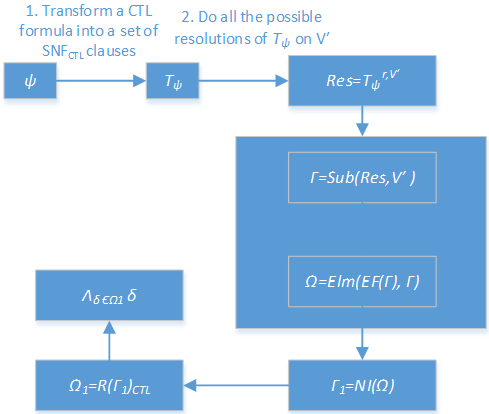
\includegraphics[width=7cm]{lct.png}\\
%  \caption{The block diagram of the algorithm}\label{Fig:lct}
%\end{figure}



\subsection{The Transform Process}
The \emph{Transform} process, denoted as $\emph{Transform}(\varphi)$, transforms the \CTL\ formula into a set of $\CTLsnf$ clauses by applying  the rules  Trans(1) to Trans(12) in~\cite{zhang2009refined}).

The \emph{transformation} of any \CTL\ formula $\varphi$ into the set $T_{\varphi}$ is a sequence $T_0, T_1,\dots, T_n=T_{\varphi}$ of sets of formulae with $T_0=\{\ALL \GLOBAL(\start \supset p), \ALL \GLOBAL(p \supset \simp(\nnf(\varphi)))\}$ such that for every $i$ ($0 \leq i< n$), $T_{i+1} = (T_i \setminus \{\psi\}) \cup R_i$~\cite{zhang2009refined}), where $p$ is a new atom not appearing in $\varphi$, $\psi$ is a formula in $T_i$ which is not in $\CTLsnf$ clause and $R_i$ is the result set of applying a matching transformation rule to $\psi$. Note that throughout the transformation, formulae are kept in negation normal form (nnf).

\begin{proposition}\label{pro:TranE}
 Let $\varphi$ be a \CTL\ formula, then $\varphi \equiv_{\tuple{V', I}} T_{\varphi}$.
\end{proposition}
\begin{proof} (sketch)
This can be proved from $T_i$ to $T_{i+1}$ $(0\leq i < n)$ by using one transformation rule on $T_i$.
We show $\varphi \equiv_{\tuple{\{p\}, {\O}}} T_0$.  Other cases are similar.

First, for every $(\Hm_1,s_1) \in \Mod(\varphi)$, \ie $(\Hm_1,s_1) \models \varphi$. We can construct an initial \Ind-model structure $\Hm_2$ which is identical to $\Hm_1$ except $L_2(s_2) = L_1(s_1) \cup \{p\}$. It is apparent that $(\Hm_2,s_2) \models T_0$ and $(\Hm_1, s_1) \lrto_{\tuple{\{p\}, {\O}}} (\Hm_2, s_2)$.

Second, for all $(\Hm_1,s_1) \in \Mod(T_0)$, it is apparent that $(\Hm_1,s_1) \models \varphi$ by the semantic of $\start$.

%We will prove this proposition from the following several aspects:
%
% (1) $\varphi \equiv_{\tuple{\{p\}, {\O}}} T_0$.

% $(\Rto)$ $\forall (\Hm_1,s_1) \in \Mod(\varphi)$, \ie $(\Hm_1,s_1) \models \varphi$. We can construct an \Ind-model structure $\Hm_2$ is identical to $\Hm_1$ except $L_2(s_2) = L_1(s_1) \cup \{p\}$. It is apparent that $(\Hm_2,s_2) \models T_0$ and $(\Hm_1, s_1) \lrto_{\tuple{\{p\}, {\O}}} (\Hm_2, s_2)$.
%
% $(\Lto)$ $\forall (\Hm_1,s_1) \in \Mod(T_0)$, it is apparent that $(\Hm_1,s_1) \models \varphi$ by the sematic of $\start$.
%
%By $\psi \rto_t R_i$ we mean using transformation rules $t$ on formula $\psi$ (the formulae $\psi$ as the
%premises of rule $t$) and obtaining the set  $R_i$ of transformation results. Let $X$ be a set of formulas
%we will show $T_i \equiv_{\tuple{V',I}} T_{i+1}$ by using the transformation rule $t$. Where $T_i= X \cup \{\psi\}$, $T_{i+1}=X \cup R_i$, $V'$ is the set of atoms introduced by $t$ and $I$ is the set of indexes introduced by $t$. (We will prove this result in $t\in \{$Trans(1), Trans(4), Trans(6)$\}$, other cases can be proved similarly.)
%
%(2) For $t$=Trans(1):\\
% $(\Rto)$ $\forall (\Hm_1,s_1) \in \Mod(T_i)$ \ie $(\Hm_1, s_1) \models X \wedge \ALL\GLOBAL(q \supset \EXIST \NEXT \varphi)$\\
% $\Rto$ $(\Hm_1,s_1)\models X$ and for every $\pi$ starting from $s_1$ and every state $s_1^j \in \pi$, $(\Hm,s_1^j) \models \neg q$ or there exists a path $\pi'$ starting from $s_1^j$ such that there exists a state $s_1^{j+1}$ such that $(s_1^j,s_1^{j+1})\in R_1$ and $(\Hm,s_1^{j+1})\models \varphi$\\
% We can construct an \Ind-model structure $\Hm_2$ is identical to $\Hm_1$ except  $[ind]_2= \bigcup_{s\in S} R_s \cup R_y$, where $R_{s_1^{j}}=\{(s_1^{j},s_1^{j+1}), (s_1^{j+1}, s_1^{j+2}),\dots\}$ and $R_y=\{(s_x,s_y)| \forall s_x \in S$ if $\forall (s_1',s_2')\in \bigcup_{s\in S} R_s, s_1'\neq s_x$ then find a unique $s_y\in S$ such that $(s_x,s_y)\in R\}$. It is apparent that $(\Hm_1, s_1) \lrto_{\tuple{{\O}, \{ind\}}} (\Hm_2, s_2)$ (let $s_2=s_1$).\\
% $\Rto$ for every path starting from $s_1$ and every state $s_1^j$ in this path, $(\Hm_2, s_1^j) \models \neg q$ or $(\Hm_2, s_1^j)\models \EXIST \NEXT \varphi_{\tuple{ind}}$ \hfill (by the semantic of $\EXIST \NEXT$)\\
% $\Rto$ $(\Hm_2, s_1) \models \ALL \GLOBAL(q \supset \EXIST_{\tuple{ind}} \NEXT \varphi )$\\
% $\Rto$ $(\Hm_2, s_1) \models X \wedge \ALL \GLOBAL(q \supset \EXIST_{\tuple{ind}} \NEXT \varphi )$
%
% $(\Lto)$ $\forall (\Hm_1,s_1) \in \Mod(T_{i+1})$ \ie $(\Hm_1,s_1) \models X \wedge \ALL \GLOBAL(q \supset \EXIST_{\tuple{ind}} \NEXT \varphi )$\\
% $\Rto$ $(\Hm_1,s_1) \models X$ and $(\Hm_1,s_1) \models \ALL \GLOBAL(q \supset \EXIST_{\tuple{ind}} \NEXT \varphi)$\\
% $\Rto$ for every path starting from $s_1$ and every state $s_1^j$ in this path, $(\Hm_1, s_1^j) \models \neg q$ or there exits a state $s'$ such that $(s_1^j, s')\in [ind]_1$ and $(\Hm_1, s') \models \varphi$ \hfill (by the semantic of $\EXIST_{\tuple{ind}} \NEXT$)\\
% $\Rto$ for every path starting from $s_1$ and every state $s_1^j$ in this path, $(\Hm_1, s_1^j) \models \neg q$ or $(\Hm_1, s_1^j) \models \EXIST \NEXT \varphi$ \hfill (by the semantic of $\EXIST \NEXT$)\\
% $\Rto$ $(\Hm_1,s_1) \models \ALL\GLOBAL(q \supset \EXIST \NEXT \varphi)$\\
% $\Rto$ $(\Hm_1, s_1) \models X \wedge \ALL\GLOBAL(q \supset \EXIST \NEXT \varphi)$\\
% It is apparent that $(\Hm_1, s_1) \lrto_{\tuple{{\O}, \{ind\}}} (\Hm_1, s_1)$.
%
%(3) For $t$=Trans(4):\\
% $(\Rto)$ $\forall (\Hm_1,s_1) \in \Mod(T_i)$, \ie $(\Hm_1,s_1) \models X \wedge \ALL\GLOBAL (q \supset \varphi_1 \vee \varphi_2)$ \\
% $\Rto$ $(\Hm_1,s_1) \models X$ and $\forall s_1'\in S, (\Hm_1,s_1') \models q \supset \varphi_1 \vee \varphi_2$\\
% $\Rto$ $(\Hm_1,s_1') \models \neg q$ or $(\Hm_1,s_1') \models \varphi_1 \vee \varphi_2$\\
% The we can construct an \Ind-model structure $\Hm_2$ as follows. $\Hm_2$ is the same with $\Hm_1$ when $(\Hm_1,s_1') \models \neg q$. When $(\Hm_1,s_1') \models q$, $\Hm_2$ is identical to $\Hm_1$ except if $(\Hm_1,s_1') \models \varphi_1$ then $L_2(s_1')= L_1(s_1')$ else $L_2(s_1') = L_1(s_1') \cup \{p\}$. It is apparent that $(\Hm_2,s_1') \models (q\supset \varphi_1 \vee p) \wedge (p \supset \varphi_2)$, then $(\Hm_2,s_1) \models T_{i+1}$ and $(\Hm_1, s_1) \lrto_{\tuple{\{p\}, {\O}}} (\Hm_2, s_2)$.
%
% $(\Lto)$ $\forall (\Hm_1, s_1) \in \Mod(T_{i+1})$, \ie $(\Hm_1,s_1) \models X \wedge \ALL\GLOBAL (q\supset \varphi_1 \vee p) \wedge \ALL\GLOBAL(p \supset \varphi_2)$. It is apparent that $(\Hm_1, s_1) \models T_i$.
%
%
%(4) For $t$=Trans(6):\\
%We prove for $\EXIST_{\tuple{ind}} \NEXT$, while for the $\ALL \NEXT$ can be proved similarly.
%
% $(\Rto)$ $\forall (\Hm_1,s_1) \in \Mod(T_i)$, \ie $(\Hm_1,s_1) \models X \wedge \ALL\GLOBAL(q \supset \EXIST_{\tuple{ind}}\NEXT \varphi)$\\
% $\Rto$ $(\Hm_1,s_1) \models X$ and $\forall s_1'\in S, (\Hm_1,s_1') \models q \supset \EXIST_{\tuple{ind}} \NEXT \varphi$\\
% $\Rto$ $(\Hm_1,s_1') \models \neg q$ or there exists a state $s'$ such that $(s_1', s') \in [ind]$ and $(\Hm_1,s') \models \varphi$ \\
% We can construct an \Ind-model structure $\Hm_2$ as follows. $\Hm_2$ is the same with $\Hm_1$ when $(\Hm_1,s_1') \models \neg q$. When $(\Hm_1,s_1') \models q$, $\Hm_2$ is identical to $\Hm_1$ except for $s'$ there is $L_2(s') = L_1(s') \cup \{p\}$. It is apparent that $(\Hm_2,s_1) \models \ALL\GLOBAL(q\supset \EXIST_{\tuple{ind}} \NEXT p) \wedge \ALL\GLOBAL(p \supset \varphi)$, $(\Hm_2,s_2) \models T_{i+1}$ and $(\Hm_1, s_1) \lrto_{\tuple{\{p\}, {\O}}} (\Hm_2, s_2)$ ($s_2=s_1$).
%
%  $(\Lto)$ $\forall (\Hm_1, s_1) \in \Mod(T_{i+1})$, \ie $(\Hm_1,s_1) \models X \wedge \ALL\GLOBAL(q\supset \EXIST_{\tuple{ind}} \NEXT p) \wedge \ALL\GLOBAL(p \supset \varphi)$. It is apparent that $(\Hm_1, s_1) \models T_i$.

\end{proof}

%This means that models of $\varphi$ and $T_{\varphi}$ are $\tuple{V', I}$-bisimular.
%, i.e. except that the label function for those atoms in $V'$ and the relations $[i]$ with $i\in I$ may be different in those models.

\begin{algorithm}[!h]
\caption{$\emph{Transform}(\varphi)$}% ??????
\label{alg:compute:transformation}
%\LinesNumbered %?????????
\KwIn{A CTL formula $\varphi$}% ????????
\KwOut{A set $T_{\varphi}$ of $\CTLsnf$ clauses and a set $V'$ of atoms}% ????
$T_{\varphi}\lto {\O}$ // the initial set of $\CTLsnf$ clauses of $\varphi$ \;
$OldT\lto \{\start \supset z, z \supset \simp(\nnf(\varphi))\}$\;
$V'\lto \{z\}$\;
\While {$OldT\neq T_{\varphi}$} {
    $OldT\lto T_{\varphi}$\;
    $R\lto {\O}$\;
    $X\lto {\O}$\;
    \If {Chose a formula $\psi\in OldT$ that does not a $\CTLsnf$ clause}{
    Using a match rule $Rl$ to transform $\psi$ into a set $R$ of $\CTLsnf$ clauses\;
    $X$ is the set of atoms introduced by using $Rl$\;
    $V' \lto V' \cup X$\;
    $T_{\varphi}\lto OldT\setminus \{\psi\} \cup R$\;
    }
}

\end{algorithm}

\begin{example}\label{examp:Tran}
By the \emph{Transform} process, the result $T_{\varphi}$ of the Example~\ref{main:examp} can be listed as follows:
\begin{align*}
& 1. \start\supset z && 2. \top \supset \neg z \vee r && 3.\top \supset \neg x\vee f \vee m\\
& 4. \top \supset \neg z \vee x \vee y && 5.\top \supset \neg y \vee p && 6.\top \supset \neg y \vee q\\
& 7. z \supset \ALL \FUTURE x && 8. y \supset \ALL \NEXT(x\vee y).
\end{align*}
Besides, the set of new atoms introduced in this process is $V'=\{x, y,x, w\}$ with $w$ is a new atom related to $z \supset \ALL \FUTURE x$. %~\cite{zhang2014resolution}.
\end{example}




\subsection{The Resolution Process}
The \emph{Resolution} process consists of computing all the possible resolutions of $T_{\varphi}$ on $V\cup V'$, denoted as $\emph{Resolution}(T_{\varphi}, V\cup V')$.
A \emph{derivation} on a set $V\cup V'$ of atoms and $T_{\varphi}$ is a sequence $T_0=T_{\varphi}, T_1, T_2$, $\dots$, $T_n=Res$ of sets of $\CTLsnf$ clauses such that $T_{i+1} = T_i \cup R_i$ for all $0\leq i < n$, where $R_i$ is a set of clauses obtained as the conclusion of the application of a resolution rule to premises in $T_i$.
Note that all $T_i$ ($0 \leq i \leq n$) are set of $\CTLsnf$ clauses.
Besides, if there is a $T_i$ containing $\start\supset \perp$ or $\top\supset \perp$, then we have $\CTLforget(\varphi, V)=\perp$.

Let $C$ be a clause and $C'$ be a clause or set of clauses. If $C$ and $C'$ are resolvable, then $res(C,C')$ is a set of $\CTLsnf$ clauses, i.e., if there is a resolution rule using $C$ and $C'$ as the premises on some given atom.
The pseudocode of \emph{Resolution} process is  shown in Algorithm~\ref{alg:compute:Res}.
\begin{proposition}\label{pro:ResE}
 Let $\varphi$ be a \CTL\ formula,
 %and $W$ be the set of new atoms introduced by resolution rules \textbf{(ERES1)} and \textbf{(ERES2)} (if any),
 then $T_{\varphi} \equiv_{\tuple{V \cup V', {\O}}} Res$.
\end{proposition}
\begin{proof}(sketch)
This can be proved from $T_i$ to $T_{i+1}$ $(0\leq i < n)$ by using one resolution rule on $T_i$.
For instance, if we can use the resolution rule (SRES1) on $\psi\subseteq T_i$ and obtain the result $R$, then we can prove $T_i \equiv T_{i+1}$ with $T_{i+1} = T_i \cup R$ as follows.

On the one hand, it is apparent that $\psi \models R$ and then $T_i \models T_{i+1}$. On the other hand, $T_i\subseteq T_{i+1}$ and then $T_{i+1} \models T_i$.

% By $\psi \rto_r R_i$ we mean using resolution rules $r$ on set $\psi$ (the formulae in $\psi$ as the premises of rule $r$) and obtaining the set $R_i$ of resolution results.
% we will show $T_i \equiv_{\tuple{V,I}} T_{i+1}$ by using the resolution rule $r$. Where $T_i= X \cup \psi$, $T_{i+1}=X \cup R_i$, $X$ be a set of $\CTLsnf$ clauses, $p$ be the proposition corresponding with literal $l$ used to do resolution in $r$.

% (1) If $\psi \rto_r R_i$ by an application of $r\in \{\textbf{(SRES1)}, \dots, \textbf{(SRES8)}, \textbf{RW1}, \textbf{RW2}\}$, then $T_i \equiv_{\tuple{\{p\}, {\O}}} T_{i+1}$.


% On one hand, it is apparent that $\psi \models R_i$ and then $T_i \models T_{i+1}$. On the other hand, $T_i\subseteq T_{i+1}$ and then $T_{i+1} \models T_i$.
%
% (2) If $\psi \rto_r R_i$ by an application of $r=$\textbf{(ERES1)},
% then $T_i \equiv_{\tuple{\{l, w_{\neg l}^{\ALL}\}, {\O}}} T_{i+1}$.

% It has been proved that $\psi \models R_i$ in~\cite{bolotov2000clausal}, then there is $T_{i+1}=T_i \cup \Lambda_{\neg l}^{\ALL}$ and  then $\forall (\Hm_1,s_1) \in \Mod(T_i= X \cup \psi)$ there is a $(\Hm_2, s_2)\in \Mod(T_{i+1}=T_i \cup \Lambda_{\neg l}^{\ALL})$ s.t. $(\Hm_1, s_1) \lrto_{\tuple{\{p, w_{\neg l}^{\ALL}\}, {\O}}} (\Hm_2, s_2)$ and vice versa by Proposition~\ref{pro:TranE}.
%
%For rule \textbf{(ERES2)} we have the same result.

\end{proof}
Proposition~\ref{pro:TranE} and Proposition~\ref{pro:ResE} mean that $\varphi \equiv_{\tuple{V \cup V', I}} Res$, this resolves a part of the problem (1).

\begin{algorithm}[!h]
\caption{$\emph{Resolution}(T,V \cup V')$}% ??????
\label{alg:compute:Res}
%\LinesNumbered %?????????
\KwIn{A set $T_{\varphi}$ of $\CTLsnf$ clauses and a set $V\cup V'$ of atoms}% ????????
\KwOut{A set $Res$ of $\CTLsnf$ clauses}% ????

$S\lto \{C | C\in T_{\varphi}$ and $\Var(C) \cap (V\cup V')= {\O}\}$\;
$\Pi\lto T\setminus S$ \;
\For {($p\in V\cup V')$} {
    $\Pi'\lto \{C \in \Pi| p\in \Var(C)\}$ \;
    $\Sigma \lto \Pi \setminus \Pi'$\;
    \For {($C\in \Pi'$ s.t. $p$ appearing in  $C$ positively)} {
        \For {($C'\in\Pi'$ s.t. $p$ appearing in  $C'$ negatively and $C$, $C'$ are resolvable)}{
            $\Sigma \lto \Sigma \cup res(C,C')$\;
            $\Pi' \lto \Pi' \cup \{C''\in res(C,C') | p\in \Var(C'')\}$\;
        }
    }
    $\Pi\lto \Sigma$\;
}

$Res\lto \Pi \cup S$\;

\end{algorithm}


\begin{example}\label{examp:Res}
The resolutions of $T_{\varphi}$ obtained from Example~\ref{examp:Tran} on $V\cup V'$ are listed as follows:
\begin{align*}
&(1) \start \supset r && (1,2,SRES 5)\\
&(2) \start \supset x \vee y && (1,4,SRES 5)\\
&(3) \top \supset \neg z \vee y \vee f \vee m && (3, 4, SRES 8)\\
&(4) y \supset \ALL\NEXT(f\vee m\vee y) && (3,8, SRES 6)\\
&(5) \top \supset \neg z \vee x \vee p && (4,5, SRES 8)\\
% \end{align*}
% \begin{align*}
&(6) \top \supset \neg z \vee x \vee q && (4,6, SRES 8)\\
&(7) y \supset \ALL\NEXT(x\vee p) && (5, 7, SRES 6)\\
&(8) y \supset \ALL\NEXT(x\vee q) && (5, 8, SRES 6)\\
&(9) \start \supset f\vee m \vee y && (3,(2), SRES 5) \\
&(10) \start \supset x \vee p && (5,(2),SRES 5) \\
&(11) \start \supset x \vee q && (6,(2), SRES 5)\\
% \end{align*}
% \begin{align*}
&(12) \top \supset p \vee \neg z \vee f \vee m && (5,(3), SRES 8)\\
&(13) \top \supset q \vee \neg z \vee f \vee m && (6,(3), SRES 8)\\
&(14) y \supset \ALL\NEXT(p \vee f\vee m) && (5, (4), SRES 6) \\
&(15) y \supset \ALL\NEXT(q \vee f\vee m) && (6, (4), SRES 6) \\
&(16) \start \supset f\vee m \vee p && (5, (9), SRES 5) \\
&(17) \start \supset f\vee m \vee q && (6, (9), SRES 5)
\end{align*}
\end{example}

\subsection{The Elimination Process}
We say that an atom appears in a formula positively if it is preceded by an even number of negative connectives.
For solving problem (2), we should pay focus on the following properties that are obtained from the transformation and resolution rules:
\begin{itemize}
  \item \textbf{(GNA)} For each atom $p \in  \Var(\varphi)$, $p$ does not positively appear in the left hand of the $\CTLsnf$ clause;
  %\item \textbf{(CNI)} for each global clause, there must be an atom $p\in V'$ appearing in the right hand negatively;
  \item \textbf{(PI)} For each atom $p\in V'$, if $p$ appears in the left hand of a $\CTLsnf$ clause, then $p$ appears positively.
\end{itemize}

The \emph{Elimination} process includes three sub-processes: \emph{Instantiate}, \emph{Connect} and \emph{Removing\_atoms}. We  describe them next.
\subsubsection{The Instantiation Process}
An \emph{instantiate formula} of a set $V''$ of atoms is a formula $\psi$ such that $\Var(\psi) \cap V'' ={\O}$.
Given a formula of the form $p \supset \psi$ with $p$ is an atom not in $V'' \cup \Var(\psi)$, if $\psi$ is an instantiate formula of set $V''$ then we say that $p$ is instantiated by $\psi$.
A key point to compute forgetting is eliminating those irrelevant atoms. For this purpose, we define the follow instantiation process.
\begin{definition}[Instantiation]\label{def:subst}
 Let $V''=V'$ and $\Gamma=Res$, then the process of instantiation is as follows:
\begin{enumerate}[(i)]
  \item for each global clause $C= \top \supset D \vee \neg p \in \Gamma$, if there is one and on one atom $p \in V''\cap \Var(C)$  and $\Var(D) \cap (V \cup V'')= {\O}$ then let $C = p \supset D$ and $V'':=V''\setminus \{p\}$;
  \item find out all the possible instantiate formulae $\varphi_1, ..., \varphi_m$ of $V \cup V''$ with $p\supset \varphi_i \in \Gamma$ ($1\leq i\leq m$);
  \item if there is $p\supset \varphi_i$ for some $i\in \{1,\dots, m\}$, then let $V'':=V''\setminus \{p\}$; %, which means $p$ is a instantiate formula;
  \item for $\bigwedge_{j=1}^n p_j \supset \varphi \in \Gamma$ ($i\in \{1,\dots, n\}$), if there is $\alpha \supset p_1,\dots, \alpha \supset p_n \in \Gamma$ and $\varphi$ is an instantiate formula of $V \cup V''$, then let $\Gamma_1 := \Gamma \cup \{\alpha \supset \varphi\}$. if $\Gamma_1\neq \Gamma$ then let $\Gamma:=\Gamma_1$ go to step (i), else if $V''$ has been changed before then go to (i) else return $V \cup V''$.
\end{enumerate}
Where $p, p_i$ ($1 \leq i\leq m$) are atoms and $\alpha$ is a conjunction of literals or $\start$.
\end{definition}

Intuitively, this process iteratively removes the atoms in $V'$ that can be represented by the formula of $\Var(\varphi) \setminus (V'' \cup V)$.
We denote this process as $\emph{Instantiate}(\Gamma, V')$. %, which can be described as the following Algorithm~\ref{alg:subn}.
 After this, we obtain a set of atoms that have not been instantiated by any instantiate formula of $V\cup V''$.

% \begin{algorithm}[!h]
% \caption{Computing $\emph{Instantiate}(\Gamma, V')$}% ??????
% \label{alg:subn}
% %\LinesNumbered %?????????
% \KwIn{A set $\Gamma$ of $\CTLsnf$ clauses $\varphi$ and $V,V'\subseteq \Ha$}% ????????
% \KwOut{A set of atoms}% ????
% Let $V''\lto V'$\;
% Let $V_1 \lto \emptyset$\;
% Let $\Gamma_1 \lto \emptyset$\;
% Let $\Gamma_2 \lto \Gamma$\;
% \While {($\Gamma_1\neq \Gamma_2$ or $V_1 \neq V''$)} {
%     $\Gamma_1\lto \Gamma_2$\;
%     $V_1 \lto V''$\;
%     \For {($C \in \Gamma_2$)} {
%         \If {($C$ is a global clause)} {
%             Let $C\lto D \vee \neg p$\;
%             \If{($p\in V''\cap \Var(C)$ and $\Var(D) \cap V==\emptyset$)} {
%                 $C\lto p\supset D$\;
%                 $V'' \lto V'' \setminus \{p\}$\;
%             }
%         }
%     }

%     \For {($C \in \Gamma_2$)} {
%         \If {($C== p\supset \varphi$ and $p\in V''$ and $\Var(\varphi) \cap V\cup V'' == \emptyset$)} {
%             $V'' \lto V'' \setminus \{p\}$\;
%         }
%     }

%     \For {($C \in \Gamma_2$)} {
%         \If {($C==\bigwedge_{j=1}^m p_j \supset \varphi$ and $\Var(\varphi) \cap V\cup V'' == \emptyset$)} {
%             \If {(there is $\alpha \supset p_1, \dots, \alpha \supset p_m \in \Gamma_2$)} {
%                 $\Gamma_2 \lto \Gamma_2 \cup \{\alpha \supset \varphi\}$\;
%             }
%         }
%     }
% }



% \Return $V \cup V''$.
% \end{algorithm}

\begin{example}\label{exa:until:sub}
By using the instantiation process on result of Example~\ref{examp:Res}, we obtain that $x$ is instantiated by $f\vee m$ at first since there is $\top \supset \neg x \vee f \vee m \in T_{\varphi}$ with $x \in V'$ and $\Var(f \vee m) \cap (V\cup V') = \emptyset$, then $V''=\{y,z\}$.

Similarly, due to $\top \supset \neg y \vee q \in T_{\varphi}$ and $y \supset \ALL\NEXT(q \vee f\vee m)\in T_{\varphi}$,  $y$ can be instantiated by $q \wedge \ALL\NEXT(q \vee f\vee m)$. And $z$ can be instantiated by $r$. Therefore $V''=\{w\}$.
%$r\wedge (f\vee m \vee q) \wedge q\wedge \ALL\NEXT(f\vee m\vee q) \wedge  (f\vee m \vee (q\wedge \ALL\NEXT(f\vee m\vee q))) \wedge \ALL\FUTURE(f \vee m)$.
That is $\emph{Instantiate}(Res, V') = V\cup \{w\}$. %, which means all the introduced atoms are instantiated.
%Let $\varphi=\ALL((p\wedge q) \UNTIL (f\vee m)) \wedge r$ and $V=\{p\}$. Then we can compute $\Sub(T_{\varphi}^{r,V \cup V'}, V)$ as follows:
%
%At first, we transform $\varphi$ into a set of $\CTLsnf$ with $V'=\{x,y,z\}$, which is listed as:
%\begin{align*}
%& 1. \start\supset z && 2. \top \supset \neg z \vee r && 3.\top \supset \neg x\vee f \vee m\\
%& 4. \top \supset \neg z \vee x \vee y && 5.\top \supset \neg y \vee p && 6.\top \supset \neg y \vee q\\
%& 7. z \supset \ALL \FUTURE x && 8. y \supset \ALL \NEXT(x\vee y).
%\end{align*}
%
%In the second, we compute all the possible resolutions on $V\cup V'$ and is listed as:
%\begin{align*}
%&(1) \start \supset r && (2) \start \supset x \vee y &&(3) \top \supset \neg z \vee y \vee f \vee m \\
%& (4) y \supset \ALL\NEXT(f\vee m\vee y) &&(5) \top \neg z \vee x \vee p && (6) \top \neg z \vee x \vee q\\
%&(7) y \supset \ALL\NEXT(x\vee p) && (8) y \supset \ALL\NEXT(x\vee q) &&(9) \start \supset f\vee m \vee y \\
%& (10) \start \supset x \vee p &&(11) \start \supset x \vee q && (12) \top \supset p \vee \neg z \vee f \vee m \\
%&(13) \top \supset q \vee \neg z \vee f \vee m && (14) y \supset \ALL\NEXT(p \vee f\vee m) &&(15) y \supset \ALL\NEXT(q \vee f\vee m) \\
%& (16) \start \supset f\vee m \vee p &&(17) \start \supset f\vee m \vee q.
%\end{align*}

%By the process of instantiation we obtain that $y$ is instantiated by $q \wedge \ALL\NEXT(p \vee f\vee m)$, $x$ is instantiated by $f\vee m$ and $z$ is instantiated by $r$. That is $\Sub(T_{\varphi}^{r,V \cup V'}, V') = V$, which means all the introduced atoms are instantiated.
\end{example}

With the instantiation operator, we guarantee that those atoms in $V\cup V''$ are indeed irrelevant \ie should be forgotten.


\subsubsection{The Connect Process}
Let $P$ be a conjunction of literals, $l$, $l_1$ be literals,
in which $\Var(l_1)\in V \cup V'$,
and $C_i$ ($i\in \{2,3,4\}$) be classical clauses.
 %Besides, by $l \supset \neg C_1 \vee C_2$ we mean the set $\{l \supset \neg C_{1,1} \vee C_2, \dots, l \supset \neg C_{1,x} \vee C_2$, where $C_{1,i}$ is a literal appearing in $C_1$.
%As we can see that those exist resolution rules cannot deduct all the possible result, so we add following new rules:
Let $A=\{true \supset \neg l \vee \neg l_1 \vee C_2, l \supset C_3\vee C_2\}$, $\alpha=P \supset ((\neg C_3 \wedge \neg C_2) \supset  (\EXIST_{\tuple{ind}}\NEXT(C_3 \wedge \neg (C_2 \vee C_4) \supset \ALL\NEXT \ALL\FUTURE(C_3 \vee C_2))))$, $\beta = P \supset ((\neg C_3 \wedge \neg C_2) \supset (\ALL\NEXT(C_3 \wedge  \neg (C_2 \vee C_4) \supset \ALL\NEXT \ALL\FUTURE(C_3 \vee C_2))))$ and $\gamma = P \supset ((\neg C_3 \wedge \neg C_2) \supset (\EXIST_{\tuple{ind}}\NEXT(C_3 \wedge  \neg (C_2 \vee C_4) \supset \EXIST_{\tuple{ind}}\NEXT \EXIST_{\tuple{ind}}\FUTURE(C_3 \vee C_2))))$, we add the following new rules, we call it \textbf{EF}-implication.
\begin{align*}
& \textbf{(EF1)} \{P\supset \ALL\FUTURE l, P\supset \EXIST_{\tuple{ind}}\NEXT (l_1 \vee C_4)\}\cup A \rto \alpha \\
%&  \qquad \rto\{P \supset ((\neg C_3 \wedge \neg C_2) \supset  (\EXIST_{\tuple{ind}}\NEXT(C_3 \wedge \neg (C_2 \vee C_4) \supset \ALL\NEXT \ALL\FUTURE(C_3 \vee C_2))))\},\\
& \textbf{(EF2)} \{P\supset \ALL\FUTURE l, P\supset \ALL \NEXT (l_1 \vee C_4)\}\cup A \rto \beta \\
%& \qquad \rto \{ P \supset ((\neg C_3 \wedge \neg C_2) \supset (\ALL\NEXT(C_3 \wedge  \neg (C_2 \vee C_4) \supset \ALL\NEXT \ALL\FUTURE(C_3 \vee C_2))))\}\\
& \textbf{(EF3)} \{P\supset \EXIST_{\tuple{ind}}\FUTURE l, P\supset \EXIST_{\tuple{ind}}\NEXT (l_1 \vee C_4)\}\cup A \rto \gamma  \\
%& \qquad \rto \{P \supset ((\neg C_3 \wedge \neg C_2) \supset (\EXIST_{\tuple{ind}}\NEXT(C_3 \wedge  \neg (C_2 \vee C_4) \supset \ALL\NEXT \ALL\FUTURE(C_3 \vee C_2))))\},\\
& \textbf{(EF4)} \{P\supset \EXIST_{\tuple{ind}}\FUTURE l, P\supset \ALL\NEXT (l_1 \vee C_4)\}\cup A \rto \gamma.
\end{align*}



By $\emph{Connect}(\emph{Instantiate}(Res, V'))$ we mean using (EF1) to (EF4) on $Res$ and replacing $P\supset \EXIST_{\tuple{ind}}\NEXT (\neg l \vee C_2 \vee C_4)$ with $P\supset \EXIST_{\tuple{ind}}\NEXT (\neg l \vee C_2 \vee C_4) \vee \alpha$ for rule (EF1), replacing $P\supset \ALL\NEXT (\neg l \vee C_2 \vee C_4)$ with $P\supset \ALL\NEXT (\neg l \vee C_2 \vee C_4) \vee \beta$ for rule (EF2) and replacing $P\supset \ALL\NEXT (\neg l \vee C_2 \vee C_4)$ with $P\supset \ALL\NEXT (\neg l \vee C_2 \vee C_4) \vee \gamma$ for other rules when $l$, $C_2$, $C_3$  and $C_4$ are instantiate formulae of  $\Sub(Res, V')$ and $\Var(l_1) \in V\cup V'$.
%This is similar with the resolution process except by those rules it will not product new resolution due to the new formulae obtained from those rules are instantiate formulae of  $\Sub(T_{\varphi}^{r,V \cup V'}, V')$.
%This process can be described as Algorithm~\ref{alg:EF}.
The reason why we specify $l$, $C_2$, $C_3$  and $C_4$ are instantiate formulae of  $\Sub(Res, V')$  will be explained later.


%\begin{algorithm}[!h]
%\caption{Computing $\emph{Connect}(\Gamma, V)$}% ??????
%\label{alg:EF}
%%\LinesNumbered %?????????
%\KwIn{A set $\Gamma$ of $\CTLsnf$ clauses, a set $A$ of $\ALL$-step clauses and a set $E$ of $\EXIST$-step clauses}% ????????
%\KwOut{A set of formulae}% ????
%
%% $C_1 :=P \supset ((\neg C_3 \wedge \neg C_2) \supset  (\EXIST_{\tuple{ind}}\NEXT(C_3 \wedge \neg (C_2 \vee C_4) \supset
%%\ALL\NEXT \ALL\FUTURE(C_3 \vee C_2))))$\;
%%$C_1' := P \supset ((\neg C_3 \wedge \neg C_2) \supset  (\ALL\NEXT(C_3 \wedge \neg (C_2 \vee C_4) \supset
%%\ALL\NEXT \ALL\FUTURE(C_3 \vee C_2))))$\;
%\For {($C \in A$)} {
%    Let $C == P \supset \ALL \FUTURE l$\;
%    \If {$(P\supset \EXIST_{\tuple{ind}}\NEXT (l_1 \vee C_4),  l \supset \neg l_1 \vee C_2, l \supset C_3\vee C_2\in \Gamma$ and $l,C_2, C_3, C_4$ are  instantiate formulae)} {
%        Replacing $P\supset \EXIST_{\tuple{ind}}\NEXT (\neg l \vee C_2 \vee C_4)$ with $P\supset \EXIST_{\tuple{ind}}\NEXT (\neg l \vee C_2 \vee C_4) \vee \alpha$\;
%    }
%    \If {$( P\supset \ALL \NEXT (l_1 \vee C_4), l \supset \neg l_1 \vee C_2, l \supset C_3\vee C_2\in \Gamma$ and $l,C_2, C_3, C_4$ are  instantiate formulae)} {
%        Replacing $P\supset \ALL\NEXT (\neg l \vee C_2 \vee C_4)$ with $P\supset \ALL\NEXT (\neg l \vee C_2 \vee C_4) \vee \beta$\;
%    }
%}
%
%
%\For {($C \in E$)} {
%    Let $C == P \supset \EXIST_{\tuple{ind}} \FUTURE l$\;
%    \If {$(P\supset \EXIST_{\tuple{ind}}\NEXT (l_1 \vee C_4),  l \supset \neg l_1 \vee C_2, l \supset C_3\vee C_2\in \Gamma \hbox{ or } P\supset \ALL \NEXT (l_1 \vee C_4), l \supset \neg l_1 \vee C_2, l \supset C_3\vee C_2\in \Gamma$ and $l,C_2, C_3, C_4$ are  instantiate formulae)} {
%        Replacing $P\supset \EXIST_{\tuple{ind}}\NEXT (\neg l \vee C_2 \vee C_4)$ with $P\supset \EXIST_{\tuple{ind}}\NEXT (\neg l \vee C_2 \vee C_4) \vee \alpha$\;
%    }
%}
%
%%Using distribution law two change $\Gamma$ into a sequence $\Gamma_1, \dots, \Gamma_m$ of sets of $\CTLsnf$ clauses\;
%\Return $\Gamma$.
%\end{algorithm}

\begin{proposition} \label{pro:EF}
Let $\Gamma=Res$, we have $\Gamma \equiv_{\tuple{V', {\O}}}\emph{Connect}(\emph{Instantiate}(\Gamma, V'))$.
\end{proposition}
\begin{proof}
It is obvious from the  \textbf{(EF1)} to \textbf{(EF4)}.

We prove the (EF1), other rules can be proved similarly.
Let $T_{i+1}=T_i \cup \{\varphi\}$, where $\{\varphi\}$ is obtained from $T_i$ by using rule (EF1) on $T_i$, \ie $\varphi =P \supset ((\neg C_3 \wedge \neg C_2) \supset  (\EXIST_{\tuple{ind}}\NEXT(C_3 \wedge \neg (C_2 \vee C_4) \supset \ALL\NEXT \ALL\FUTURE(C_3 \vee C_2))))$.
It is apparent that $T_{i+1} \models T_i$ and $T_i \models P\supset \EXIST_{\tuple{ind}}\NEXT (\neg l \vee C_2 \vee C_4)$.
We will show that for all $(\Hm, s_0) \in \Mod(T_i)$ there is an initial Ind-structure $(\Hm',s_0')$ such that $(\Hm',s_0') \models T_{i+1}$ and $(\Hm',s_0') \lrto_{\tuple{V', {\O}}} (\Hm, s_0)$

$\forall (\Hm, s) \models T_i$ we suppose $(\Hm, s) \models P \wedge \neg C_3 \wedge \neg C_2$ and $(\Hm, s_1)\models C_3 \wedge \neg C_2 \wedge \neg C_4$ with $(s, s_1) \in [ind]$ (due to other case can be proved easily).
Then we have $(\Hm, s) \nvDash l$ (by $(\Hm, s) \models l \supset C_3 \vee C_2$) and $(\Hm,s_1) \models l_1$ (by $(\Hm, s) \models P\supset \EXIST_{\tuple{ind}}\NEXT (l_1 \vee C_4)$).
If $(\Hm,s_1) \nvDash \ALL\NEXT \ALL\FUTURE(C_3 \vee C_2)$ then we have $(\Hm, s_1) \models l$ due to $(\Hm, s) \models \ALL\GLOBAL(l\supset C_3 \vee C_2)$ and $(\Hm, s)\models \ALL\FUTURE l$.
And then $(\Hm, s_1) \models \neg l_1$ by $(\Hm,s) \models \ALL \GLOBAL(l\supset \neg l_1 \vee C_2)$.
it is a contradiction.
Then $(\Hm,s_1) \models \ALL\NEXT \ALL\FUTURE(C_3 \vee C_2)$.

%By Proposition~\ref{pro:TranE} we have $\forall (\Hm, s) \in \Mod(\varphi)$ there is an initial Ind-structure $(\Hm',s')$ such that $(\Hm', s')\models T_{\varphi}$ and $(\Hm,s) \lrto_{\tuple{V_F, \emptyset}} (\Hm, s)$.

\end{proof}


\subsubsection{The Removing\_atoms process}
For eliminating those irrelevant atoms, we define the following \emph{Removing\_atoms} operator.
\begin{definition}[Removing\_atoms]\label{def:Elm}
%\textbf{(Elimination)}
Let $T$ be a set of formulae, $C \in T$ and $V$ a set of atoms, then the Removing\_atoms operator is defined as:
$$ \emph{Removing\_atoms}(C, V)=\left\{
\begin{aligned}
\top, && if\ \Var(C) \cap V \neq {\O} \\
C, && else.
\end{aligned}
\right.
$$
\end{definition}
Intuitively, if the formula $C$ contains at least one of atoms in $V$ then let $\emph{Removing\_atoms}(C, V)$ be true, else be $C$ itself.
For convenience, for any set $T$ of formula we have $\emph{Removing\_atoms}(T, V) = \{\emph{Removing\_atoms}(r, V) | r \in T\}$.



\begin{proposition}\label{pro:elm}
Let $V''=V \cup V'$, $\Gamma=\emph{Instantiate}(Res, V')$ and $\Gamma_1=\emph{Removing\_atoms}$ $(\emph{Connect}(\Gamma), \Gamma)$, then  $\Gamma_1\equiv_{\tuple{V'', {\O}}} Res$ and $\Gamma_1 \equiv_{\tuple{V'', I}} \varphi$.
\end{proposition}
\begin{proof}(stretch)
Note that for each clause $C = T \supset H$ in $\emph{Connect}(\Gamma)$, if $\Gamma \cap \Var(C) \neq \emptyset$ then there must be an atom $p\in \Gamma \cap \Var(H)$. It is apparent that $\emph{Connect}(\Gamma) \models \Gamma_1$. We  show that  for all $(\Hm, s_0) \in \Mod(\Gamma_1)$ there is a $(\Hm', s_0)$ such that $(\Hm', s_0) \models \emph{Connect}(\Gamma)$ and $(\Hm, s_0) \lrto_{\tuple{\Gamma, \emptyset}} (\Hm', s_0)$.
Let $C = T \supset H$ in $\emph{Connect}(\Gamma)$ with $\Gamma \cap \Var(C) \neq \emptyset$,
for all $(\Hm, s_0) \in \Mod(\Gamma_1)$ we construct $(\Hm', s_0)$ s.t. $(\Hm,s_0) \lrto_{\Gamma} (\Hm', s_0)$ and $(\Hm', s_0) \models C$ by adding or deleting some atoms in $\Gamma$ to the $L'(s')$ with $s'\in S'$.
%as $(\Hm, s_0)$ except
%We will proof this proposition from the following two points.
%  for each $s\in S$, if $(\Hm, s) \nvDash T$ then $L'(s) = L(s)$, else:
% \begin{enumerate}[(i)]
%   \item if $(\Hm,s) \models H$, then $L'(s) = L(s)$;
%   \item else if $(\Hm, s) \models T$ with $p \in \Var(H)\cap \Gamma$, then if $p$ appearing in $H$ negatively, then if $C$ is a global (or an initial) clause then let $L'(s) = L(s) \setminus \{p\}$ else let $L'(s^*) = L(s^*) \setminus \{p\}$ for (each (if $C$ is an $\ALL$-step or $\ALL$-sometime clause)) $s^* \in \pi_s$, else if $C$ is a global (or an initial) clause then let $L'(s) = L(s) \cup \{p\}$ else let $L'(s^*) = L(s^*) \cup \{p\}$ for (each (if $C$ is a $\ALL$-step or $\ALL$-sometime clause)) $s^* \in \pi_s$. Where $s^*$ is a next or future state of $s$ (it depends on the type of the clause: if the clause is a $X$-step ($X\in \{\ALL, \EXIST\}$) clause then $s^*$ is the next state, else if the clause is a $X$-sometime clause then $s^*$ is a future state).
%  % \item for other clause $C=Q\supset H$ with $p\in \Var(H)\cap \Gamma$, we can do it as (ii).
% \end{enumerate}

% It is apparent that $(\Hm, s_0) \lrto_{\tuple{\Gamma, \emptyset}} (\Hm', s_0)$, we will show that $(\Hm', s_0) \models \emph{Connect}(\Gamma)$ from the following two points:
% \begin{enumerate}[(1)]
%   \item For (i), it is apparent $(\Hm', s_0) \models C$;
%   \item For (ii) talked-above, we show it from the form of $\CTLsnf$ clauses. Supposing $C_1$ and $C_2$ are instantiate formula of $\Gamma$:
%   \begin{enumerate}[(a)]
%     \item If $C$ is a global clause, i.e. $C=\top \supset p \vee C_1$ with $C_1$ is a disjunction of literals (we suppose $p$ appearing in $C$ positively). If there is a $C'=\top \supset \neg p \vee C_2 \in \emph{Connect}(\Gamma)$, then there is $\top \supset C_1 \vee C_2 \in \emph{Connect}(\Gamma)$ by the resolution ($(\Hm,s) \models C_2$ due to we have suppose $(\Hm,s) \nvDash C$). It is apparent that $(\Hm', s_0) \models C \wedge C'$.
%     \item If $C = T \supset \EXIST_{\tuple{ind}}\NEXT (p \vee C_1)$.
%     %We talk about the case that $(\Hm,s)\models T$ and $(\Hm,s)\nvDash \EXIST_{\tuple{ind}}\NEXT (p \vee C_1)$
%         If there is a $C'=T' \supset \EXIST_{\tuple{ind}}\NEXT( \neg p \vee C_2) \in \emph{Connect}(\Gamma)$, then there is $T\wedge T' \supset \EXIST_{\tuple{ind}}\NEXT(C_1 \vee C_2) \in \emph{Connect}(\Gamma)$  by the resolution ($(\Hm,s) \models \EXIST_{\tuple{ind}}\NEXT C_2$ due to we have suppose $(\Hm,s) \nvDash C$). It is apparent that $(\Hm', s_0) \models C \wedge C'$.
%     \item Other cases can be proved similarly.
%   \end{enumerate}

%  % \item  (iii) can be proved as (ii) due to the fact we point at the beginning.
% \end{enumerate}
% Therefore, we have $\Gamma_1\equiv_{\tuple{V'', {\O}}} Res$  by Proposition~\ref{pro:VI:div} and Proposition~\ref{pro:EF}.

% And then $\Gamma_1 \equiv_{\tuple{V'', I}} \varphi$ follows.
\end{proof}


\begin{example}\label{examp:remA}
After removing the clauses that include atoms in $V=\{p\}$, the following clauses are left:
\begin{align*}
& \start\supset z &&  \top \supset \neg z \vee r\\
& \top \supset \neg x\vee f \vee m &&  \top \supset \neg z \vee x \vee y \\
&  \top \supset \neg y \vee p &&  \top \supset \neg y \vee q\\
&  z \supset \ALL \FUTURE x &&   y \supset \ALL \NEXT(x\vee y) \\
& \start \supset r && \start \supset x \vee y \\
& \top \supset \neg z \vee y \vee f \vee m && y \supset \ALL\NEXT(f\vee m\vee y)\\
& \top \supset \neg z \vee x \vee q && y \supset \ALL\NEXT(x\vee q) \\
&  \start \supset f\vee m \vee y && \start \supset x \vee q \\
& \top \supset q \vee \neg z \vee f \vee m && y \supset \ALL\NEXT(q \vee f\vee m) \\
& \start \supset f\vee m \vee q
\end{align*}
\end{example}

In this case, if we do not specify $l$, $C_2$, $C_3$  and $C_4$ are instantiate formulae of  $\Sub(Res, V')$, it is easy to check that all results including  $P\supset \EXIST_{\tuple{ind}}\NEXT (\neg l \vee C_2 \vee C_4)$ and $P\supset \ALL \NEXT (\neg l \vee C_2 \vee C_4)$ obtained from the \emph{Connect} process will be deleted in the Removing\_atoms process.

\subsection{Remove the Index and Start}
%The $\emph{Removing\_index}(\Gamma)$ process is to change the set $\Gamma$ of formulas into a set of formulas without the index by using the equations in Proposition~\ref{pro:In2NI}.
%The following proposition is important for our algorithm since ... .
The $\emph{Removing\_index}(\emph{RemA})$ process is to change the set $\emph{RemA}$ obtained above into a set of formulas without the index by using the equations in Proposition~\ref{pro:In2NI}.
%The following proposition is important for our algorithm since ... .
\begin{proposition}\label{pro:In2NI}
Let $P$, $P_i$ and $\varphi_i$ be \CTL\ formulas, then
\begin{enumerate}[(i)]
  \item $\bigwedge_{i=1}^n (P\supset \EXIST_{\tuple{ind}} \NEXT \varphi_i)  \equiv_{\tuple{\emptyset, \{ind\}}} P\supset \EXIST \NEXT \bigwedge_{i=1}^n \varphi_i$,
  \item $\bigwedge_{i=1}^n (P_i\supset \EXIST_{\tuple{ind}} \NEXT \varphi_i) \equiv_{\tuple{\emptyset, \{ind\}}} \bigwedge_{e \in 2^{\{0,\dots, n\}} \setminus \{\emptyset\}}(\bigwedge_{i\in e}P_i\supset \EXIST \NEXT (\bigwedge_{i\in e}\varphi_i))$,
  \item $\bigwedge_{i=1}^n (P\supset \EXIST_{\tuple{ind}} \FUTURE \varphi_i)  \equiv_{\tuple{\emptyset, \{ind\}}} P\supset \bigvee\EXIST\FUTURE (\varphi_{j_1} \wedge \EXIST\FUTURE(\varphi_{j_2} \wedge \EXIST\FUTURE(\dots \wedge \EXIST\FUTURE \varphi_{j_n})))$, where $(j_1, \dots, j_n)$ are sequences of all elements in $\{0, \dots, n\}$,
  \item $P\supset (C \vee \EXIST_{\tuple{ind}} \NEXT \varphi_1) \wedge P \supset \EXIST_{\tuple{ind}} \NEXT \varphi_2 \equiv_{\tuple{\emptyset, \{ind\}}} P \supset ((C \wedge \EXIST \NEXT \varphi_2) \vee \EXIST \NEXT (\varphi_1 \wedge \varphi_2))$,
  \item $P\supset (C \vee \EXIST_{\tuple{ind}} \NEXT \varphi_1) \vee P \supset \EXIST_{\tuple{ind}} \NEXT \varphi_2 \equiv_{\tuple{\emptyset, \{ind\}}} P \supset (C \vee \EXIST \NEXT (\varphi_1 \vee \varphi_2))$.
\end{enumerate}
\end{proposition}
\begin{proof}
(i)  For all $(\Hm, s_0) \in \Mod(\bigwedge_{i=1}^n (P\supset \EXIST_{\tuple{ind}} \NEXT \varphi_i))$ there exists $(s_0, s_1)\in [ind]$ such that $(\Hm, s_1) \models \varphi_1$, \dots, $(\Hm, s_1) \models \varphi_n$, then there is $(s_0, s_1)\in R$ s.t. $(\Hm, s_1) \models \bigwedge_{i=1}^n \varphi_i$, i.e. $(\Hm, s_0) \models P\supset \EXIST \NEXT \bigwedge_{i=1}^n \varphi_i$.

For each $(\Hm, s_0) \in \Mod(P\supset \EXIST \NEXT \bigwedge_{i=1}^n \varphi_i)$, we suppose there is $(s_0, s_1)\in R$ s.t. $(\Hm, s_1) \models \bigwedge_{i=1}^n \varphi_i$. It is easy to construct an initial \Ind-model $(\Hm', s_0)$ such that $(\Hm', s_0)$ is identical to $(\Hm, s_0)$ except the $(s_0, s_1) \in [ind]$, i.e. $(\Hm, s_0) \lrto_{\tuple{\emptyset, \{ind\}}} (\Hm', s_0)$.

(ii) (If part) For any model $(\Hm,s_0)$ of the left side of the equation if there is $(\Hm,s_0) \models \bigwedge_{i=1}^m P_{j_i}$ with $j_i \in \{1, \dots, n\}$ and $1\leq m \leq n$, then there is a next state $s_1$ of $s_0$ with $(s_0, s_1) \in [ind]$ such that $(\Hm, s_1) \models \bigwedge_{i=1}^m \varphi_{j_i}$. By the definition of $[ind]$, we have $(s_0, s_1) \in R$ and then $(\Hm, s_0) \models \bigwedge_{i=1}^m P_{j_i} \supset \EXIST \NEXT (\bigwedge_{i=1}^m P_{j_i} \varphi_{j_i})$. The other side can be similarly proved as (i).

(iii) (Only if part) For any model $(\Hm,s_0)$ of the right side of the equation if there is $(\Hm,s_0) \models P$ then there exists a path $\pi_{s_0}$ such that $\varphi_i \in \pi_{s_0}$ ($1\leq i \leq n$). This means we can construct an initial \Ind-model $(\Hm', s_0)$ such that $(\Hm', s_0)$ is identical to $(\Hm, s_0)$ except for each $(s_j, s_{j+1})$ of $\pi_{s_0}$ there is $(s_j, s_{j+1}) \in [ind]$ $(0\leq j)$. It is easy to check $(\Hm', s_0) \models \bigwedge_{i=1}^n (P\supset \EXIST_{\tuple{ind}} \FUTURE \varphi_i)$ and  $(\Hm, s_0) \lrto_{\tuple{\emptyset, \{ind\}}} (\Hm', s_0)$.  The other side can be shown similarly as in (ii).

Other results can be proved similarly.
\end{proof}

The following proposition follows from Proposition~\ref{pro:In2NI}.

\begin{proposition}\label{lem:No:Ind}
\textbf{(NI-BRemain)}
Let $I$ be the set of indexes appearing in $\emph{RemA}$, then
we have $\emph{RemA}\equiv_{\tuple{{\O}, I}} \emph{Removing\_index}(\emph{RemA})$.
\end{proposition}
% \begin{proof}
% It is easy checking that from the definition of $\emph{Removing\_index}$ and Proposition~\ref{pro:In2NI}.
% \end{proof}


%\subsection{Remove the \start}
In our Example~\ref{examp:remA} we do not need such  process since there is no index in the set of formulae.
%\subsection{Remove the \start}
Let $T$ be a set of $\CTLsnf$ clauses, then we define the following operator:
\begin{align*}
&T_{\CTL} = \{C|C'\in T\ \mbox{and}\ C = D \ \mbox{if}\ C' \mbox{is the form}\\
& \ALL\GLOBAL(\start\supset D), \mbox{else}\ C= C'\}.
\end{align*}
Then $T \equiv T_{\CTL}$ by $\varphi \equiv \ALL \GLOBAL (\start \supset \varphi)$~\cite{bolotov2000clausal}.


The last step of our algorithm is to eliminate all the atoms in $V'$ which has been introduced in the \emph{Transform} process.

Let $\Gamma=\emph{Instantiate}(Res, V')$ and $\Gamma_1=\emph{Removing\_atoms} (\emph{Connect}(\Gamma))$, then $\emph{Replacing\_atoms}(\emph{Removing\_index}(\Gamma_1))$ is obtained from $\emph{Removing\_index}(\Gamma_1)$ by doing the following three steps for each $p\in (V'\setminus \Gamma)$:
\begin{itemize}
  \item replacing each $p\supset \varphi_1\vee \dots \vee p \supset \varphi_n$ with $p \supset \bigvee_{i=1}^n \varphi_i$;
  \item replacing $p\supset \varphi_{1}\wedge \dots \wedge p \supset \varphi_{m}$ with $\varphi_j$ are instantiate formulae of  $\Gamma$ $(j \in \{1,\dots, m\})$ with $p \supset \psi$, where $\psi=\bigwedge_{j=1}^{m} \varphi_{j}$ and $p$ do not appear in $\varphi_j$, .
  \item For any formula $C\in \Gamma_1$, replacing every $p$ in $C$ with $\psi$.
\end{itemize}
%Where $\NI(S)$ means do $\NI(e)$ for each $e\in S$ with $S$ is a set of sets of $\CTLsnf$ clause.
Recall that any atom in $V'$ introduced in the Transform process is a name of the sub-formula of $\varphi$~\cite{bolotov2000clausal}. Apparently, this process is just a process of replacing each atom with an equivalent formula. Then we have:
\begin{proposition}\label{pro:replaceA}
Let $\Gamma_1=\emph{Instantiate}(Res, V')$, $\Gamma_2 =\emph{Removing\_atoms}$ $(\emph{Connect}(\Gamma_1), \Gamma_1)$ and $\Gamma_3 = \emph{Replacing\_atoms}(\emph{Removing\_index}(\Gamma_2))$, then $\Gamma_2  \equiv_{\tuple{V'\setminus \Gamma_1, I}} \Gamma_3$ and $\varphi \equiv_{\tuple{V\cup V', \emptyset}}$ $(\Gamma_3)_{CTL}$.
\end{proposition}
%\begin{proof}
%For each $p$ talked above is a name of the formula $\psi$. %, \ie $p \lrto \psi$.
%Then $\Gamma_2  \equiv_{\tuple{(V'\setminus \Gamma_1), {\O}}} \Gamma_3$, and then $\Gamma_2 \equiv_{\tuple{V\cup V', I}} \Gamma_3$  by (V) of Proposition~\ref{div}.
%
%Therefore, $\varphi \equiv_{\tuple{V\cup V',{\O}}} (\Gamma_3)_{CTL}$ by Proposition~\ref{pro:elm} and the definitions of $\emph{Removing\_index}$ and $T_{\CTL}$.
%\end{proof}


\begin{example}\label{exa:replace:sub}
By using the \emph{Replacing\_atoms} process on result of Example~\ref{examp:remA} directly since there is no index in those clauses, we obtain that $x$ is replaced by $f\vee m$. Then $y$ is replaced by $q \wedge \ALL\NEXT(q \vee f\vee m)$ and $z$ is replaced by $r\wedge (f\vee m \vee q) \wedge (f\vee m \vee (q\wedge \ALL\NEXT(f\vee m\vee q))) \wedge \ALL\FUTURE(f \vee m)$.
\end{example}



\subsection{An Example for the Connect Process}
In order to show the necessity of the Connect process, we give the following example.
\begin{example}
Let $\psi=\ALL\FUTURE(p \wedge q) \wedge \EXIST \NEXT \neg p$ and $V=\{p\}$.
By the processes Transform and Resolution, we can obtain $V'=\{f,z,w\}$ and the following set $Res$ of $\CTLsnf$ clauses.
\begin{align*}
& \start \supset z && z \supset \ALL\FUTURE f && z \supset  \EXIST_{\tuple{ind}} \NEXT \neg p \\
& \top \supset \neg f \vee p && \top \supset \neg f \vee q && z \supset \EXIST_{\tuple{ind}} \NEXT \neg f
\end{align*}

 According to our Algorithm~\ref{alg:compute:forgetting:by:Resolution}, we have $\emph{Instantiate}(Res,V')=\{p,w\}$ since $f$ can be instantiated by $q$ and $z$ can be instantiated by $\ALL\FUTURE f$.

On the one hand, in the \emph{Connect} process, by using \textbf{(EF1)} rule on the $Res$ we have $\alpha=z \supset (\neg q \supset  (\EXIST_{\tuple{ind}}\NEXT (q \supset \ALL\NEXT \ALL\FUTURE q )))$ and replace $z \supset \EXIST_{\tuple{ind}} \NEXT \neg f \in Res$ with $z \supset \EXIST_{\tuple{ind}} \NEXT \neg f \vee \alpha$ since $l$, $C_2$, $C_3$ and $C_4$ are instantiate formulae.
Apparently, $z \supset \EXIST_{\tuple{ind}} \NEXT \neg f \vee \alpha \equiv z \supset q \vee \EXIST_{\tuple{ind}} \NEXT(\neg f \vee \neg q \vee \ALL\NEXT \ALL\FUTURE q)$.

After the \emph{Removing\_atoms} process, we have the following set \emph{RemA} of formulae:
\begin{align*}
& \start \supset z && z \supset \ALL\FUTURE f \\
&  \top \supset \neg f \vee q && z \supset q \vee \EXIST_{\tuple{ind}} \NEXT(\neg f \vee \neg q \vee \ALL\NEXT \ALL\FUTURE q)
\end{align*}

Removing the indexes appearing in the \emph{RemA}, we obtain the following set $\NI$:
 \begin{align*}
& \start \supset z && z \supset \ALL\FUTURE f \\
&  \top \supset \neg f \vee q && z \supset q \vee \EXIST \NEXT(\neg f \vee \neg q \vee \ALL\NEXT \ALL\FUTURE q)
\end{align*}

Replacing the atoms in $V'$ that have been instantiated, i.e. $f$ is replaced with $q$ and $z$ is  replaced with $\ALL\FUTURE q \wedge (q \vee \EXIST \NEXT(\neg q \vee \ALL\NEXT \ALL\FUTURE q))$, we have
\[
\emph{Rp}= \{\start \supset  \ALL\FUTURE q \wedge (q \vee \EXIST \NEXT(\neg q \vee \ALL\NEXT \ALL\FUTURE q))\}.
\]

As all the formulas $\cal F$ in the $T_{\varphi}$ are the form $\ALL\GLOBAL \cal F$, hence we have:
\[
\emph{Rp}_{\CTL} = \{\ALL\FUTURE q \wedge (q \vee \EXIST \NEXT(\neg q \vee \ALL\NEXT \ALL\FUTURE q))\}
\]
i.e. $\emph{ERes}(\varphi, V) = \ALL\FUTURE q \wedge (q \vee \EXIST \NEXT(\neg q \vee \ALL\NEXT \ALL\FUTURE q))$.
In this case, we can easily check that $\emph{ERes}(\varphi, V) \equiv_{\tuple{V, \emptyset}} \varphi$.


On the other hand, if we do not using the \emph{Connect} process, we can easily obtain the result of $\emph{ERes}$, i.e. $\emph{ERes}(\varphi, V) = \ALL\FUTURE q \wedge  \EXIST \NEXT(\neg q)$.
It is apparent that $\emph{ERes}(\varphi, V) \not\equiv_{\tuple{V, \emptyset}} \varphi$. This can proved by model $(\Hm,s_0)$ as in Figure~\ref{Fig:models} since $(\Hm, s_0) \models \varphi$ and $(\Hm, s_0) \not \models \emph{ERes}(\varphi, V)$.
\begin{figure}[ht!]
  \centering
   %Requires \usepackage{graphicx}
  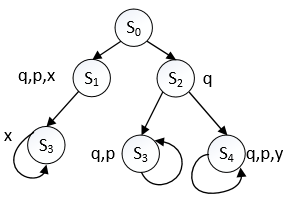
\includegraphics[width=5cm]{models.png}\\
  \caption{A model $(\Hm, s_0)$ of $\varphi$}\label{Fig:models}
\end{figure}
\end{example}

This example shows why we introduce the \textbf{EF}-implication rules. Intuitively, the result of replacing the atoms that have been instantiated in $V'$ with an instantiate formula is stronger than our method, because by the \emph{Removing\_atoms} process, we have removed some clauses, such as $C= \top \supset \neg f \vee p$, that contain $f$. The original one is $f \supset p \wedge q$, but after removing $C$ we only obtain  $f \supset q$. In this example, there is a clause $z \supset \EXIST \NEXT \neg f \in Res$, after replacing $f$ with $q$, we obtain $z \supset \EXIST \NEXT \neg q$. However, if we do not remove $C$ (i.e. $f \supset p \wedge q$), then we have $z \supset \EXIST \NEXT (\neg q \vee \neg p)$, this is weaker than $z \supset \EXIST \NEXT \neg q$.
In fact, for any model $(\Hm, s_0)$ of $\varphi$, it might be the case that $q \in L(s)$ for all next states $s$ of $s_0$ and if there is $q \in L(s)$ for all next states s, then there must be a next state $s$ of $s_0$ with $p \not \in L(s)$ s.t. for all next state $s'$ of $s$ there is $(\Hm, s')\models \ALL\FUTURE q$ (see Fig.~\ref{Fig:models}).
%This is what the meaning of the \emph{Connect} process.

\subsection{Soundness and Complexity of the Algorithm}
If a formula contains no index for its existential quantifier and \start, only initial \MPK-structures are considered to be candidate models. Because in such a case, it is a \CTL\ formula.%In the case that formula does not include index, we use model structure $\Hm=(S,R,L, s_0)$ to interpret formula instead of \Ind-model structure.
%Therefore it is apparent that $\forall (\Hm,s_0) \in \Mod(\varphi)$ there is a $(\Hm',s_0') \in \Mod(\Gamma_1)$ such that $(\Hm,s_0) \lrto_{V \cup V'} (\Hm',s_0')$ and vice versa.

The soundness means that the result $\emph{ERes}(\varphi,V)$ obtained from our Algorithm is $\CTLforget(\varphi, V)$, i.e. output the result of forgetting $V$ from $\varphi$ when input $\varphi$ and $V$ to Algorithm~\ref{alg:compute:forgetting:by:Resolution}.
\begin{theorem}[Soundness]\label{thm:Res_based:V_CTLforget}
Let $V''=V \cup V'$ and $\Gamma_1=\emph{ERes}(\varphi,V)$, then %R(\NI(\Elm(\EXIST\FUTURE(\Gamma),\Gamma)))_{\CTL}$, then
\begin{enumerate}[(i)]
\item $\CTLforget(\varphi, V'') \equiv \Gamma_1$;
\item $\CTLforget(\varphi, V) \equiv \Gamma_1$.
\end{enumerate}
\end{theorem}
\begin{proof}
(i) ($\Rto$) For all $(\Hm,s_0) \in \Mod(\CTLforget(\varphi, V''))$ there exists $(\Hm',s_0') \in \Mod(\varphi)$ s.t. $(\Hm,s_0) \lrto_{V''} (\Hm', s_0')$ by the definition of $\CTLforget$, and then there exists $(\Hm_1, s_1) \in \Mod(\Gamma_1)$ s.t. $(\Hm_1,s_1) \lrto_{V''} (\Hm', s_0')$ by Proposition~\ref{pro:replaceA}. Hence, $(\Hm,s_0) \lrto_{V''} (\Hm_1,s_1)$ since  $\lrto$ is an equivalence relation.
Therefore, $(\Hm,s_0) \models \Gamma_1$ since $\IR(\Gamma_1, V'')$ and Theorem~\ref{thm:V-bisimulation:EQ}.

 ($\Lto$)  For all $(\Hm_1, s_1) \in \Mod(\Gamma_1)$ there exists $(\Hm',s_0') \in \Mod(\varphi)$ s.t. $(\Hm_1,s_1) \lrto_{V''} (\Hm', s_0')$ by Proposition~\ref{pro:replaceA}. Hence, $(\Hm_1, s_1) \models \CTLforget(\varphi, V'')$ since $\IR(\CTLforget(\varphi, V''), V'')$ and $\varphi \models \CTLforget(\varphi, V'')$.

 (ii) It is obtained from (i) since $\IR(\varphi, V')$.
\end{proof}

Then we can obtain the result of forgetting of Example~\ref{exa:until:sub}:
\begin{align*}
& \CTLforget(\varphi, \{p\}) \equiv r\wedge (f\vee m \vee q)  \wedge  \ALL\FUTURE(f \vee m) \wedge\\
& (f\vee m \vee (q\wedge \ALL\NEXT(f\vee m\vee q)))  \wedge \ALL\GLOBAL((q\wedge \ALL\NEXT(f\vee m\vee q)\\
& \supset \ALL\NEXT(f\vee m \vee (q\wedge \ALL\NEXT(f\vee m\vee q))))).
\end{align*}


\begin{proposition}\label{pro:complexity}
Let $\varphi$ be a CTL formula and $V \subseteq \Ha$.
The time and space complexity of Algorithm~\ref{alg:compute:forgetting:by:Resolution} are $O((m+1)2^{4(n+n')}$ where $|\Var(\varphi)|=n$, $|V'|=n'$ ($V'$ is set of atoms introduced in transformation) and $m$ is the number of indices introduced during transformation.
\end{proposition}
% \begin{proof}
% It follows from the lines 19-31 of the algorithm~\ref{alg:compute:forgetting:by:Resolution}, which is to compute all the possible resolution.
% The possible number of $\CTLsnf$ clauses under the give $V$, $V'$ and $Ind$ is $(m+1)2^{4(n+n')}+(m*(n+n')+n+n'+1)2^{2(n+n')+1})$.
% \end{proof}

Indeed, $m$ is at most the number of  temporal  operators in $\varphi$.
That is, the computational complexity of our algorithm only depends on the number of atoms and temporal operators in $\varphi$.
Although it is exponential, it is more efficient than that of the model-based algorithm in~\cite{renyansfirstpaper}, which not only depends on the number of atoms in $\Ha$ but also the number of states.

\section{Related work}
%\subsection{Resolution-based satisfiability of \CTL}
Deciding satisfiability with resolution calculus in Propositional Linear Temporal Logic (PLTL) was introduced in~\cite{fisher1991resolution} and further discussed in~\cite{fisher1997normal,fisher2001clausal}. The main idea is to transform PLTL formulas into the a normal form, called Separated Normal Form (SNF) by introducing a new connective \start\ that holds only at the beginning of time.

Later,  resolution-based satisfiability in \CTL\ was proposed by Bolotov in~\cite{bolotov2000clausal}  and then further refined by Zhang in~\cite{zhang2009refined,zhang2014resolution}.
In those papers, the main idea is also to transform \CTL\ formulas into a normal form $\CTLsnf$.
But as \CTL\ is branching time temporal logic, they introduce ``indices" besides \start\ for that purpose. All in all, a complete set of transformation and resolution rules had been proposed for both PLTL and \CTL. It has been shown that this transformation is satisfiability-preserving, which also holds for the result obtained from using the resolution rules on the normal form.

%\subsection{Using Resolution to Compute Forgetting}
Other resolution procedures which are similar to Second-order quantifier elimination, has been used to compute the forgetting or uniform interpretation in propositional logic~\cite{Yisong:2015:arx} and Modal logic~\cite{herzig2008uniform}. In those case, the formula is required to be in a particular form-``CNF" (the definition of CNF in Modal logic can be found in~\cite{herzig2008uniform}).

 As aforementioned, the normal form used here for resolution is an extension of \CTL\ with \start\ and ``index".
 %In this article, we propose $\tuple{V,I}$-bisimulation to deal with the ``index" problem.
%In order to eliminate those atoms introduced in the transformation, we proposed the four EF-implication rules.

\section{Conclusion and Future Work}
This paper proposed a resolution-based algorithm to compute the forgetting in \CTL.
Our method extend the resolution calculus in~\cite{zhang2014resolution} by adding processes that remove  irrelevant atoms and which transforming the result back into \CTL\ formula.
For this purpose, a new type of binary bisimulation relation, called $\tuple{V,I}$-bisimulation, has been defined to bridge the gap between \CTL\ and $\CTLsnf$. Besides, for connecting the next state and future state we proposed four EF-implication rules. These rules yield the result of the original resolution, and our proposal of Replacing\_atoms also ensure that we obtain the correct result.
Finally, we proved that our algorithm is sound, i.e., return the result of forgetting some set of atoms from a \CTL\ formula.
%, and the time and space complexity of Algorithm~\ref{alg:compute:forgetting:by:Resolution} are $O((m+1)2^{4(n+n')}$.
Examples show how to compute forgetting using our algorithm.
Moreover, our resolution-based method is more efficient than that of model-base in~\cite{renyansfirstpaper}.

%In the future we will implement this algorithm (part of it has been implemented actually).
As for the future research, a Prolog implementation is currently under development, and we are planning to evaluate its practical aspects.\footnote{https://github.com/fengrenyan/Resolution-proof-CTL/blob/master/main-code.pl.}
Moreover, as for the theory, we are planning to carry out a parameterised complexity analysis on our resolution calculus.
%Besides, applying the defined methods to similar formalism.

%\section*{Acknowledgments}

% \clearpage
% \appendix
% \section{Supplementary Material: Proof Appendix}

% % \begin{lemma}\label{lem:B:relations}
% %   Let  $\Hb_0, \Hb_1,\ldots$ be the ones in the definition of section 3.1.
% %   Then,  for each $i\ge 0$,
% %   \begin{enumerate}[(i)]
% %      \item $\Hb_{i+1}\subseteq \Hb_i$;
% %      \item there is a (smallest) $k\ge 0$ such that $\Hb_{k+1}=\Hb_k$;
% %      \item $\Hb_i$ is reflexive, symmetric and transitive.
% %   \end{enumerate}
% % \end{lemma}
% % \begin{proof}
% % See~\cite{renyansfirstpaper}.
% % %   (i)
% % %   Base: it is clear for $i=0$ by the above definition.

% % %   Step: suppose it holds for $i=n$, i.e., $\Hb_{n+1}\subseteq\Hb_n$. \\
% % %   $(s,s')\in\Hb_{n+2}$\\
% % %   $\Rto$ (a) $(s,s')\in  \Hb_0$,
% % %     (b) for every $(s,s_1)\in R$, there is $(s',s_1')\in R'$
% % %      such that $(s_1,s_1')\in \Hb_{n+1}$, and
% % %     (c)  for every $(s',s_1')\in R'$, there is $(s,s_1)\in R$
% % %     such that $(s_1,s_1')\in \Hb_{n+1}$\\
% % %   $\Rto$ (a) $(s,s')\in  \Hb_0$,
% % %   (b) for every $(s,s_1)\in R$, there is $(s',s_1')\in R'$
% % %      such that $(s_1,s_1')\in \Hb_{n}$ by inductive assumption, and
% % %   (c)  for every $(s',s_1')\in R'$, there is $(s,s_1)\in R$
% % %     such that $(s_1,s_1')\in \Hb_{n}$ by inductive assumption\\
% % %   $\Rto$ $(s,s')\in \Hb_{n+1}$.

% % %   (ii) and (iii) are evident from (i) and the definition of $\Hb_i$.
% % \end{proof}


% % \noindent\textbf{Lemma}~\ref{lem:equive}  The relation $\lrto_V$ is an equivalence relation.
% % \begin{proof}
% % See~\cite{renyansfirstpaper}.
% % % It is clear from Lemma~\ref{lem:B:relations} (ii) such that there is a $k \geq $ 0 where $\Hb_k = \Hb_{k+1}$ which is  $\lrto_V$, and it is reflexive, symmetric and transitive by (iii).
% % \end{proof}


% % \noindent\textbf{Proposition}~\ref{div}
% % Let $i\in \{1,2\}$, $V_1,V_2\subseteq\cal A$
% % and ${\cal K}_i=({\cal M}_i,s_i)~(i=1,2,3)$ be \MPK-structures (Ind-structures)
% %  such that
% % ${\cal K}_1\lrto_{V_1}{\cal K}_2$ and ${\cal K}_2\lrto_{V_2}{\cal K}_3$.
% %  Then:
% %  \begin{enumerate}[(i)]
% %   \item ${\cal K}_1\lrto_{V_1\cup V_2}{\cal K}_3$;
% %   \item If $V_1 \subseteq V_2$ then ${\cal K}_1 \lrto_{V_2} {\cal K}_2$.
% %  \end{enumerate}
% % \begin{proof}
% % See~\cite{renyansfirstpaper}.
% % % In order to distinguish the relations $\Hb_0, \Hb_1, \dots$ for different set $V \subseteq \Ha$, by $\Hb_i^V$ we mean the relation $\Hb_1, \Hb_2, \dots$ for $V \subseteq \Ha$.
% % % Denote as $\Hb_0, \Hb_1, \dots$ when the underlying set $V$ is clear from the context. Moreover, for the ease of notation, we will refer to $\lrto_V$ by $\Hb$ (i.e., without subindex).

% % % The following property show our result directly.
% % % Let $V\subseteq\cal A$
% % % %${\cal M}_i=(S_i,R_i,L_i,s_0^i)~(i=1,2)$ be model structures
% % % and ${\cal K}_i=({\cal M}_i,s_i)~(i=1,2)$ be \MPK-structures.
% % % Then $({\cal K}_1,{\cal K}_2)\in\cal B$ if and only if
% % %   \begin{enumerate}[(a)]
% % %     \item $L_1(s_1)- V = L_2(s_2)- V$,
% % %     \item for every $(s_1,s_1')\in R_1$, there is $(s_2,s_2')\in R_2$
% % %     such that $({\cal K}_1',{\cal K}_2')\in \Hb$, and
% % %     \item for every $(s_2,s_2')\in R_2$, there is $(s_1,s_1')\in R_1$
% % %     such that $({\cal K}_1',{\cal K}_2')\in \Hb$,
% % %   \end{enumerate}
% % %  where ${\cal K}_i'=({\cal M}_i,s_i')$ with $i\in\{1,2\}$.

% % %  We prove it from the following two aspects:

% % %  $(\Rto)$
% % % (a) It is apparent that $L_1(s_1)- V = L_2(s_2)- V$;
% % % (b) %We will show that for each $(s_1, s_1') \in R_1$, there is a $(s_2, s_2')\in R_2$ such that $({\cal K}_1', {\cal K}_2') \in \Hb$.
% % % $({\cal K}_1, {\cal K}_2) \in \Hb$ iff $({\cal K}_1, {\cal K}_2) \in \Hb_i$ for all $i \geq 0$, then for each $(s_1, s_1') \in R_1$, there is a $(s_2, s_2')\in R_2$  such that  $({\cal K}_1', {\cal K}_2') \in \Hb_{i-1}$ for all $i > 0$ and then $L_1(s_1')- V = L_2(s_2')- V$. Therefore, $({\cal K}_1', {\cal K}_2') \in \Hb$.
% % % (c) %We will show that for each $(s_2, s_2') \in R_1$, there is a $(s_1, s_1')\in R_2$ such that $({\cal K}_1', {\cal K}_2') \in \Hb$.
% % %  This is similar with (b).

% % % $(\Lto)$ Apparently, $L_1(s_1)- V = L_2(s_2)- V$ implies that $(s_1, s_2) \in \Hb_0$;
% % % (b) implies that for every $(s_1,s_1')\in R_1$, there is $(s_2,s_2')\in R_2$
% % %     such that $({\cal K}_1',{\cal K}_2')\in \Hb_i$ for all $i \geq 0$;
% % % (c) implies that for every $(s_2,s_2')\in R_2$, there is $(s_1,s_1')\in R_1$
% % %     such that $({\cal K}_1',{\cal K}_2')\in \Hb_i$ for all $i \geq 0$\\
% % % $\Rto$ $({\cal K}_1, {\cal K}_2) \in \Hb_i$ for all $i \geq 0$\\
% % % $\Rto$ $({\cal K}_1,{\cal K}_2)\in\cal B$.

% % % (i) Let ${\cal M}_i=(S_i,R_i,L_i,s_i)~(i=1,2,3)$, $s_1 \lrto_{V_1} s_2$ via a binary relation $\Hb$, and $s_2 \lrto_{V_2} s_3$ via a binary relation $\Hb''$. Let $\Hb' = \{(w_1, w_3)| (w_1, w_2)\in \Hb$ and $(w_2, w_3)\in \Hb_2\}$. It's apparent that $(s_1, s_3) \in \Hb'$. We prove $\Hb'$ is a $V_1 \cup V_2$-bisimulation containing $(s_1, s_3)$ from the (a), (b) and (c) of the previous steps of $X$-bisimulation (where $X$ is a set of atoms). For all $(w_1, w_3) \in \Hb'$:
% % % \begin{enumerate}[(a)]
% % %   \item there is $w_2 \in S_2$ such that $(w_1,w_2)\in \Hb$ and $(w_2, w_3)\in \Hb''$, and $\forall q \notin V_1$, $q \in L_1(w_1)$ iff $q \in L_2(w_2)$ by $w_1 \lrto_{V_1} w_2$ and $\forall q' \notin V_2$, $q'\in L_2(w_2)$ iff $q'\in L_3(w_3)$ by $w_2 \lrto_{V_2} w_3$. Then we have $\forall r\notin V_1 \cup V_2$, $r \in L_1(w_1)$ iff $r \in L_3(w_3)$.
% % %   \item if $(w_1, u_1) \in \Hr_1$, then $\exists u_2\in S_2$ such that $(w_2, u_2) \in \Hr_2$ and $(u_1,u_2)\in \Hb$ (due to $(w_1,w_2)\in \Hb$ and $(w_2, w_3) \in \Hb''$ by the definition of $\Hb'$); and then $\exists u_3 \in S_3$ such that $(w_3, u_3) \in \Hr_3$ and $(u_2, u_3) \in \Hb''$, hence $(u_1, u_3) \in \Hb'$ by the definition of $\Hb'$.
% % %   \item if $(w_3, u_3) \in \Hr_3$, then $\exists u_2\in S_2$ such that $(w_2, u_2) \in \Hr_2$ and $(u_2, u_3) \in \Hb_2$; and then $\exists u_1 \in S_1$ such that $(w_1, u_1) \in \Hr_1$ and $(u_1, u_2) \in \Hb$, hence $(u_1, u_3) \in \Hb'$ by the definition of $\Hb'$.
% % % \end{enumerate}

% % % (ii)  Let ${\cal K}_{i, j}=(\Hm_i, s_{i,j})$ and $(s_{i, k}, s_{i, k+1}) \in R_i$ mean that $s_{i, k+1}$ is the $(k+2)$-th node in the path
% % %  $(s_i, s_{i, 1}, s_{i,2}, \dots , s_{i, k+1}, \dots)$ ($i=1,2$).
% % % We will show that $({\cal K}_1, {\cal K}_2) \in \Hb_n^{V_2}$ for all $n \ge 0$ inductively.

% % % Base: $L_1(s_1) - V_1 = L_2(s_2) - V_1$\\
% % % $\Rto$ $\forall q \in {\cal A} - V_1$ there is $q \in L_1(s_1)$ iff $q \in L_2(s_2)$\\
% % % $\Rto$ $\forall q \in {\cal A} - V_2$ there is $q \in L_1(s_1)$ iff $q \in L_2(s_2)$ due to $V_1 \subseteq V_2$\\
% % % $\Rto$ $L_1(s_1) - V_2 = L_2(s_2) - V_2$, i.e.,\ $({\cal K}_1, {\cal K}_2) \in \Hb_0^{V_2}$.

% % % Step: Supposing that $({\cal K}_1, {\cal K}_2) \in \Hb_i^{V_2}$ for all $0 \leq i \leq k$ ($k > 0)$, we will show $({\cal K}_1, {\cal K}_2) \in \Hb_{k+1}^{V_2}$.
% % % \begin{enumerate} [(a)]
% % %   \item It is apparent that $L_1(s_1) - V_2 = L_2(s_2) - V_2$ by base.
% % %   \item $\forall (s_1, s_{1,1}) \in R_1$, we will show that there is a $(s_2, s_{2, 1}) \in R_2$ s.t.\ $({\cal K}_{1,1}, {\cal K}_{2,1})\in \Hb_k^{V_2}$. $({\cal K}_{1,1}, {\cal K}_{2,1})\in \Hb_{k-1}^{V_2}$ by inductive assumption, we need only to prove the following points:\\
% % %       (a) $\forall (s_{1, k}, s_{1, k+1}) \in R_1$ there is a $(s_{2, k}, s_{2, k+1})\in R_2$ s.t.\ $({\cal K}_{1,k+1}, {\cal K}_{2,k+1})\in \Hb_0^{V_2}$ due to $({\cal K}_{1,1}, {\cal K}_{2,1})\in \Hb_{k}^{V_1}$. It is easy to see that $L_1(s_{1, k+1}) - V_1 = L_1(s_{2, k+1}) - V_1$, then there is $L_1(s_{1, k+1})- V_2 = L_1(s_{2, k+1}) - V_2$. Therefore, $({\cal K}_{1,k+1}, {\cal K}_{2,k+1})\in \Hb_0^{V_2}$.\\
% % %       (b) $\forall (s_{2, k}, s_{2, k+1}) \in R_1$ there is a $(s_{1, k}, s_{1, k+1}) \in R_1$ s.t.\ $({\cal K}_{1,k+1}, {\cal K}_{2,k+1})\in \Hb_0^{V_2}$ due to $({\cal K}_{1,1}, {\cal K}_{2,1})\in \Hb_{k}^{V_1}$. This can be proved as (a).
% % %   \item $\forall (s_2, s_{2,1}) \in R_1$, we will show that there is a $(s_1, s_{1, 1}) \in R_2$ s.t.\ $({\cal K}_{1,1}, {\cal K}_{2,1})\in \Hb_k^{V_2}$. This can be proved as (ii).
% % % \end{enumerate}
% % \end{proof}


% % \noindent\textbf{Theorem}\ref{thm:V-bisimulation:EQ}
% % Let $V\subseteq\cal A$, ${\cal K}_i~(i=1,2)$ be two \MPK-structures such that
% %   ${\cal K}_1\lrto_V{\cal K}_2$ and $\phi$ a formula with $\IR(\phi,V)$. Then
% %   ${\cal K}_1\models\phi$ if and only if ${\cal K}_2\models\phi$.
% % \begin{proof}
% % See~\cite{renyansfirstpaper}.
% % % This theorem can be proved by inducting on the formula $\phi$ and supposing $\Var(\phi) \cap V = \Empty$.
% % % Let ${\cal K}_1 = (\Hm, s)$ and ${\cal K}_2 = (\Hm', s')$.

% % % %Here we only prove the only-if direction. The other direction can be similarly proved.

% % % \textbf{Case} $\phi = p$ where $p \in \Ha - V$:\\
% % % $(\Hm, s) \models \phi$ iff $p\in L(s)$  \hfill  (by the definition of satisfiability) \\
% % % $\LRto$ $p \in L'(s')$ \hfill ($s \lrto_V s'$)\\
% % % $\LRto$ $(\Hm', s') \models \phi$

% % % \textbf{Case} $\phi = \neg \psi$:\\
% % % $(\Hm, s) \models \phi$ iff $(\Hm, s) \nvDash \psi$ \\
% % % $\LRto$ $(\Hm', s') \nvDash \psi$  \hfill   (induction hypothesis)\\
% % % $\LRto$ $(\Hm', s') \models \phi$

% % % \textbf{Case} $\phi = \psi_1 \vee \psi_2$:\\
% % % $(\Hm, s) \models \phi$\\
% % % $\LRto$ $(\Hm, s) \models \psi_1$ or $(\Hm, s) \models \psi_2$\\
% % % $\LRto$ $(\Hm', s') \models \psi_1$ or $(\Hm', s') \models \psi_2$   \hfill  (induction hypothesis)\\
% % % $\LRto$ $(\Hm', s') \models \phi$

% % % \textbf{Case} $\phi = \EXIST \NEXT \psi$:\\
% % % %By Lemma~\ref{V_path}, we assume there are two paths $\pi = s, s_1, ...$ and $\pi' = s', s_1', ...$ such that $\pi \lrto_V \pi'$.\\
% % % $\Hm, s \models \phi$ \\
% % % $\LRto$ There is a path $\pi = (s, s_1, ...)$ such that $\Hm, s_1 \models \psi$\\
% % % $\LRto$ There is a path $\pi' = (s', s_1', ...)$ such that $\pi \lrto_V \pi'$ \hfill   ($s \lrto_V s'$, Proposition~\ref{div})\\
% % % $\LRto$ $s_1 \lrto_V s_1'$  \hfill ($\pi \lrto_V \pi'$)\\
% % % $\LRto$ $(\Hm', s_1') \models \psi$  \hfill  (induction hypothesis)\\
% % % $\LRto$ $(\Hm', s') \models \phi$

% % % \textbf{Case} $\phi = \EXIST \GLOBAL \psi$:\\
% % % $\Hm, s \models \phi$ \\
% % % $\LRto$ There is a path $\pi =(s=s_0, s_1, ...)$ such that for each $i \geq 0$ there is $(\Hm, s_i) \models \psi$\\
% % % $\LRto$ There is a path $\pi' = (s'=s_0', s_1', ...)$ such that $\pi \lrto_V \pi'$   \hfill ($s \lrto_V s'$, Proposition~\ref{div})\\
% % % $\LRto$ $s_i \lrto_V s_i'$ for each $i \geq 0$ \hfill ($\pi \lrto_V \pi'$)\\
% % % $\LRto$ $(\Hm', s_i') \models \psi$ for each $i \geq 0$  \hfill  (induction hypothesis)\\
% % % $\LRto$ $(\Hm', s') \models \phi$

% % % \textbf{Case} $\phi = \EXIST [\psi_1 \UNTIL \psi_2]$:\\
% % % %\textbf{Case} $\varphi = \MPE \FUTURE \psi$:
% % % $\Hm, s \models \phi$ \\
% % % $\LRto$ There is a path $\pi= (s=s_0, s_1, ...)$ such that there is $i \geq 0$ such that $(\Hm, s_i) \models \psi_2$, and for all $0 \leq j < i$, $(\Hm, s_j) \models \psi_1$\\
% % % $\LRto$ There is a path $\pi' = (s=s_0', s_1', ...)$ such that $\pi \lrto_V \pi'$  \hfill  ($s \lrto_V s'$, Proposition~\ref{div})\\
% % % $\LRto$ $(\Hm', s_i') \models \psi_2$, and for all $0 \leq j < i$ $(\Hm', s_j') \models \psi_1$   \hfill   (induction hypothesis)\\
% % % $\LRto$ $(\Hm', s') \models \phi$
% % \end{proof}

% \noindent\textbf{Proposition}~\ref{pro:TranE}
%  Let $\varphi$ be a \CTL\ formula, then $\varphi \equiv_{\tuple{V', I}} T_{\varphi}$.
% \begin{proof} (sketch)
% This can be proved from $T_i$ to $T_{i+1}$ $(0\leq i < n)$ by using one transformation rule on $T_i$.
% We will prove this proposition from the following several aspects:

% (1) $\varphi \equiv_{\tuple{\{p\}, {\O}}} T_0$.

% $(\Rto)$ $\forall (\Hm_1,s_1) \in \Mod(\varphi)$, \ie $(\Hm_1,s_1) \models \varphi$. We can construct an \Ind-model structure $\Hm_2$ is identical to $\Hm_1$ except $L_2(s_2) = L_1(s_1) \cup \{p\}$. It is apparent that $(\Hm_2,s_2) \models T_0$ and $(\Hm_1, s_1) \lrto_{\tuple{\{p\}, {\O}}} (\Hm_2, s_2)$.

% $(\Lto)$ $\forall (\Hm_1,s_1) \in \Mod(T_0)$, it is apparent that $(\Hm_1,s_1) \models \varphi$ by the sematic of $\start$.

% By $\psi \rto_t R_i$ we mean using transformation rules $t$ on formula $\psi$ (the formulae $\psi$ as the
% premises of rule $t$) and obtaining the set  $R_i$ of transformation results. Let $X$ be a set of formulas
% we will show $T_i \equiv_{\tuple{V',I}} T_{i+1}$ by using the transformation rule $t$. Where $T_i= X \cup \{\psi\}$, $T_{i+1}=X \cup R_i$, $V'$ is the set of atoms introduced by $t$ and $I$ is the set of indexes introduced by $t$. (We will prove this result in $t\in \{$Trans(1), Trans(4), Trans(6)$\}$, other cases can be proved similarly.)

% (2) For $t$=Trans(1):\\
% $(\Rto)$ $\forall (\Hm_1,s_1) \in \Mod(T_i)$ \ie $(\Hm_1, s_1) \models X \wedge \ALL\GLOBAL(q \supset \EXIST \NEXT \varphi)$\\
% $\Rto$ $(\Hm_1,s_1)\models X$ and for every $\pi$ starting from $s_1$ and every state $s_1^j \in \pi$, $(\Hm,s_1^j) \models \neg q$ or there exists a path $\pi'$ starting from $s_1^j$ such that there exists a state $s_1^{j+1}$ such that $(s_1^j,s_1^{j+1})\in R_1$ and $(\Hm,s_1^{j+1})\models \varphi$\\
% We can construct an \Ind-model structure $\Hm_2$ is identical to $\Hm_1$ except  $[ind]_2= \bigcup_{s\in S} R_s \cup R_y$, where $R_{s_1^{j}}=\{(s_1^{j},s_1^{j+1}), (s_1^{j+1}, s_1^{j+2}),\dots\}$ and $R_y=\{(s_x,s_y)| \forall s_x \in S$ if $\forall (s_1',s_2')\in \bigcup_{s\in S} R_s, s_1'\neq s_x$ then find a unique $s_y\in S$ such that $(s_x,s_y)\in R\}$. It is apparent that $(\Hm_1, s_1) \lrto_{\tuple{{\O}, \{ind\}}} (\Hm_2, s_2)$ (let $s_2=s_1$).\\
% $\Rto$ for every path starting from $s_1$ and every state $s_1^j$ in this path, $(\Hm_2, s_1^j) \models \neg q$ or $(\Hm_2, s_1^j)\models \EXIST \NEXT \varphi_{\tuple{ind}}$ \hfill (by the semantic of $\EXIST \NEXT$)\\
% $\Rto$ $(\Hm_2, s_1) \models \ALL \GLOBAL(q \supset \EXIST_{\tuple{ind}} \NEXT \varphi )$\\
% $\Rto$ $(\Hm_2, s_1) \models X \wedge \ALL \GLOBAL(q \supset \EXIST_{\tuple{ind}} \NEXT \varphi )$

% $(\Lto)$ $\forall (\Hm_1,s_1) \in \Mod(T_{i+1})$ \ie $(\Hm_1,s_1) \models X \wedge \ALL \GLOBAL(q \supset \EXIST_{\tuple{ind}} \NEXT \varphi )$\\
% $\Rto$ $(\Hm_1,s_1) \models X$ and $(\Hm_1,s_1) \models \ALL \GLOBAL(q \supset \EXIST_{\tuple{ind}} \NEXT \varphi)$\\
% $\Rto$ for every path starting from $s_1$ and every state $s_1^j$ in this path, $(\Hm_1, s_1^j) \models \neg q$ or there exits a state $s'$ such that $(s_1^j, s')\in [ind]_1$ and $(\Hm_1, s') \models \varphi$ \hfill (by the semantic of $\EXIST_{\tuple{ind}} \NEXT$)\\
% $\Rto$ for every path starting from $s_1$ and every state $s_1^j$ in this path, $(\Hm_1, s_1^j) \models \neg q$ or $(\Hm_1, s_1^j) \models \EXIST \NEXT \varphi$ \hfill (by the semantic of $\EXIST \NEXT$)\\
% $\Rto$ $(\Hm_1,s_1) \models \ALL\GLOBAL(q \supset \EXIST \NEXT \varphi)$\\
% $\Rto$ $(\Hm_1, s_1) \models X \wedge \ALL\GLOBAL(q \supset \EXIST \NEXT \varphi)$\\
% It is apparent that $(\Hm_1, s_1) \lrto_{\tuple{{\O}, \{ind\}}} (\Hm_1, s_1)$.

% (3) For $t$=Trans(4):\\
% $(\Rto)$ $\forall (\Hm_1,s_1) \in \Mod(T_i)$, \ie $(\Hm_1,s_1) \models X \wedge \ALL\GLOBAL (q \supset \varphi_1 \vee \varphi_2)$ \\
% $\Rto$ $(\Hm_1,s_1) \models X$ and $\forall s_1'\in S, (\Hm_1,s_1') \models q \supset \varphi_1 \vee \varphi_2$\\
% $\Rto$ $(\Hm_1,s_1') \models \neg q$ or $(\Hm_1,s_1') \models \varphi_1 \vee \varphi_2$\\
% The we can construct an \Ind-model structure $\Hm_2$ as follows. $\Hm_2$ is the same with $\Hm_1$ when $(\Hm_1,s_1') \models \neg q$. When $(\Hm_1,s_1') \models q$, $\Hm_2$ is identical to $\Hm_1$ except if $(\Hm_1,s_1') \models \varphi_1$ then $L_2(s_1')= L_1(s_1')$ else $L_2(s_1') = L_1(s_1') \cup \{p\}$. It is apparent that $(\Hm_2,s_1') \models (q\supset \varphi_1 \vee p) \wedge (p \supset \varphi_2)$, then $(\Hm_2,s_1) \models T_{i+1}$ and $(\Hm_1, s_1) \lrto_{\tuple{\{p\}, {\O}}} (\Hm_2, s_2)$.

% $(\Lto)$ $\forall (\Hm_1, s_1) \in \Mod(T_{i+1})$, \ie $(\Hm_1,s_1) \models X \wedge \ALL\GLOBAL (q\supset \varphi_1 \vee p) \wedge \ALL\GLOBAL(p \supset \varphi_2)$. It is apparent that $(\Hm_1, s_1) \models T_i$.


% (4) For $t$=Trans(6):\\
% We prove for $\EXIST_{\tuple{ind}} \NEXT$, while for the $\ALL \NEXT$ can be proved similarly.

% $(\Rto)$ $\forall (\Hm_1,s_1) \in \Mod(T_i)$, \ie $(\Hm_1,s_1) \models X \wedge \ALL\GLOBAL(q \supset \EXIST_{\tuple{ind}}\NEXT \varphi)$\\
% $\Rto$ $(\Hm_1,s_1) \models X$ and $\forall s_1'\in S, (\Hm_1,s_1') \models q \supset \EXIST_{\tuple{ind}} \NEXT \varphi$\\
% $\Rto$ $(\Hm_1,s_1') \models \neg q$ or there exists a state $s'$ such that $(s_1', s') \in [ind]$ and $(\Hm_1,s') \models \varphi$ \\
% We can construct an \Ind-model structure $\Hm_2$ as follows. $\Hm_2$ is the same with $\Hm_1$ when $(\Hm_1,s_1') \models \neg q$. When $(\Hm_1,s_1') \models q$, $\Hm_2$ is identical to $\Hm_1$ except for $s'$ there is $L_2(s') = L_1(s') \cup \{p\}$. It is apparent that $(\Hm_2,s_1) \models \ALL\GLOBAL(q\supset \EXIST_{\tuple{ind}} \NEXT p) \wedge \ALL\GLOBAL(p \supset \varphi)$, $(\Hm_2,s_2) \models T_{i+1}$ and $(\Hm_1, s_1) \lrto_{\tuple{\{p\}, {\O}}} (\Hm_2, s_2)$ ($s_2=s_1$).

%  $(\Lto)$ $\forall (\Hm_1, s_1) \in \Mod(T_{i+1})$, \ie $(\Hm_1,s_1) \models X \wedge \ALL\GLOBAL(q\supset \EXIST_{\tuple{ind}} \NEXT p) \wedge \ALL\GLOBAL(p \supset \varphi)$. It is apparent that $(\Hm_1, s_1) \models T_i$.

% \end{proof}


% \noindent\textbf{Proposition}~\ref{pro:ResE}
%  Let $\varphi$ be a \CTL\ formula,
%  %and $W$ be the set of new atoms introduced by resolution rules \textbf{(ERES1)} and \textbf{(ERES2)} (if any),
%  then $T_{\varphi} \equiv_{\tuple{V \cup V', {\O}}} Res$.

% \begin{proof}(sketch)
% This can be proved from $T_i$ to $T_{i+1}$ $(0\leq i < n)$ by using one resolution rule on $T_i$.


% By $\psi \rto_r R_i$ we mean using resolution rules $r$ on set $\psi$ (the formulae in $\psi$ as the premises of rule $r$) and obtaining the set $R_i$ of resolution results.
% we will show $T_i \equiv_{\tuple{V,I}} T_{i+1}$ by using the resolution rule $r$. Where $T_i= X \cup \psi$, $T_{i+1}=X \cup R_i$, $X$ be a set of $\CTLsnf$ clauses, $p$ be the proposition corresponding with literal $l$ used to do resolution in $r$.

% (1) If $\psi \rto_r R_i$ by an application of $r\in \{\textbf{(SRES1)}, \dots, \textbf{(SRES8)}, \textbf{RW1}, \textbf{RW2}\}$, then $T_i \equiv_{\tuple{\{p\}, {\O}}} T_{i+1}$.


% On one hand, it is apparent that $\psi \models R_i$ and then $T_i \models T_{i+1}$. On the other hand, $T_i\subseteq T_{i+1}$ and then $T_{i+1} \models T_i$.

% (2) If $\psi \rto_r R_i$ by an application of $r=$\textbf{(ERES1)},
% then $T_i \equiv_{\tuple{\{l, w_{\neg l}^{\ALL}\}, {\O}}} T_{i+1}$.

% It has been proved that $\psi \models R_i$ in~\cite{bolotov2000clausal}, then there is $T_{i+1}=T_i \cup \Lambda_{\neg l}^{\ALL}$ and  then $\forall (\Hm_1,s_1) \in \Mod(T_i= X \cup \psi)$ there is a $(\Hm_2, s_2)\in \Mod(T_{i+1}=T_i \cup \Lambda_{\neg l}^{\ALL})$ s.t. $(\Hm_1, s_1) \lrto_{\tuple{\{p, w_{\neg l}^{\ALL}\}, {\O}}} (\Hm_2, s_2)$ and vice versa by Proposition~\ref{pro:TranE}.

% For rule \textbf{(ERES2)} we have the same result.

% \end{proof}

% \noindent\textbf{Proposition}~\ref{pro:elm}
% Let $V''=V \cup V'$, $\Gamma=\emph{Instantiate}(Res, V')$ and $\Gamma_1=\emph{Removing\_atoms}$ $(\emph{Connect}(\Gamma), \Gamma)$, then  $\Gamma_1\equiv_{\tuple{V'', {\O}}} Res$ and $\Gamma_1 \equiv_{\tuple{V'', I}} \varphi$.
% \begin{proof}
% Take note the fact that for each clause $C = T \supset H$ in $\emph{Connect}(\Gamma)$, if $\Gamma \cap \Var(C) \neq \emptyset$ then there must be an atom $p\in \Gamma \cap \Var(H)$. It is apparent that $\emph{Connect}(\Gamma) \models \Gamma_1$, we will show $\forall (\Hm, s_0) \in \Mod(\Gamma_1)$ there is a $(\Hm', s_0)$ such that $(\Hm', s_0) \models \emph{Connect}(\Gamma)$ and $(\Hm, s_0) \lrto_{\tuple{\Gamma, \emptyset}} (\Hm', s_0)$.
% Let $C = T \supset H$ in $\emph{Connect}(\Gamma)$ with $\Gamma \cap \Var(C) \neq \emptyset$,
% $\forall (\Hm, s_0) \in \Mod(\Gamma_1)$ we construct $(\Hm', s_0)$ as $(\Hm, s_0)$ except
% %We will proof this proposition from the following two points.
%  for each $s\in S$, if $(\Hm, s) \nvDash T$ then $L'(s) = L(s)$, else:
% \begin{enumerate}[(i)]
%   \item if $(\Hm,s) \models H$, then $L'(s) = L(s)$;
%   \item else if $(\Hm, s) \models T$ with $p \in \Var(H)\cap \Gamma$, then if $p$ appearing in $H$ negatively, then if $C$ is a global (or an initial) clause then let $L'(s) = L(s) \setminus \{p\}$ else let $L'(s^*) = L(s^*) \setminus \{p\}$ for (each (if $C$ is an $\ALL$-step or $\ALL$-sometime clause)) $s^* \in \pi_s$, else if $C$ is a global (or an initial) clause then let $L'(s) = L(s) \cup \{p\}$ else let $L'(s^*) = L(s^*) \cup \{p\}$ for (each (if $C$ is a $\ALL$-step or $\ALL$-sometime clause)) $s^* \in \pi_s$. Where $s^*$ is a next or future state of $s$ (it depends on the type of the clause: if the clause is a $X$-step ($X\in \{\ALL, \EXIST\}$) clause then $s^*$ is the next state, else if the clause is a $X$-sometime clause then $s^*$ is a future state).
%  % \item for other clause $C=Q\supset H$ with $p\in \Var(H)\cap \Gamma$, we can do it as (ii).
% \end{enumerate}

% It is apparent that $(\Hm, s_0) \lrto_{\tuple{\Gamma, \emptyset}} (\Hm', s_0)$, we will show that $(\Hm', s_0) \models \emph{Connect}(\Gamma)$ from the following two points:
% \begin{enumerate}[(1)]
%   \item For (i), it is apparent $(\Hm', s_0) \models C$;
%   \item For (ii) talked-above, we show it from the form of $\CTLsnf$ clauses. Supposing $C_1$ and $C_2$ are instantiate formula of $\Gamma$:
%   \begin{enumerate}[(a)]
%     \item If $C$ is a global clause, i.e. $C=\top \supset p \vee C_1$ with $C_1$ is a disjunction of literals (we suppose $p$ appearing in $C$ positively). If there is a $C'=\top \supset \neg p \vee C_2 \in \emph{Connect}(\Gamma)$, then there is $\top \supset C_1 \vee C_2 \in \emph{Connect}(\Gamma)$ by the resolution ($(\Hm,s) \models C_2$ due to we have suppose $(\Hm,s) \nvDash C$). It is apparent that $(\Hm', s_0) \models C \wedge C'$.
%     \item If $C = T \supset \EXIST_{\tuple{ind}}\NEXT (p \vee C_1)$.
%     %We talk about the case that $(\Hm,s)\models T$ and $(\Hm,s)\nvDash \EXIST_{\tuple{ind}}\NEXT (p \vee C_1)$
%         If there is a $C'=T' \supset \EXIST_{\tuple{ind}}\NEXT( \neg p \vee C_2) \in \emph{Connect}(\Gamma)$, then there is $T\wedge T' \supset \EXIST_{\tuple{ind}}\NEXT(C_1 \vee C_2) \in \emph{Connect}(\Gamma)$  by the resolution ($(\Hm,s) \models \EXIST_{\tuple{ind}}\NEXT C_2$ due to we have suppose $(\Hm,s) \nvDash C$). It is apparent that $(\Hm', s_0) \models C \wedge C'$.
%     \item Other cases can be proved similarly.
%   \end{enumerate}

%  % \item  (iii) can be proved as (ii) due to the fact we point at the beginning.
% \end{enumerate}
% Therefore, we have $\Gamma_1\equiv_{\tuple{V'', {\O}}} Res$  by Proposition~\ref{pro:VI:div} and Proposition~\ref{pro:EF}.

% And then $\Gamma_1 \equiv_{\tuple{V'', I}} \varphi$ follows.
% \end{proof}


% \noindent\textbf{proposition}~\ref{pro:complexity}
% Let $\varphi$ be a CTL formula and $V \subseteq \Ha$.
% The time and space complexity of Algorithm~\ref{alg:compute:forgetting:by:Resolution} are $O((m+1)2^{4(n+n')}$. Where $|\Var(\varphi)|=n$, $|V'|=n'$ ($V'$ is set of atoms introduced in transformation) and $m$ is the number of indices introduced during transformation.
% \begin{proof}
% It follows from the lines 19-31 of the algorithm~\ref{alg:compute:forgetting:by:Resolution}, which is to compute all the possible resolution.
% The possible number of $\CTLsnf$ clauses under the give $V$, $V'$ and $Ind$ is $(m+1)2^{4(n+n')}+(m*(n+n')+n+n'+1)2^{2(n+n')+1})$.
% \end{proof}

%% The file kr.bst is a bibliography style file for BibTeX 0.99c
\clearpage
\bibliographystyle{kr}
\bibliography{ijcai20}

\end{document}

